% Requires in the preamble:
% \usepackage{amsmath,amssymb}
% \usepackage{tikz,pgfplots}
% \pgfplotsset{compat=1.18}

\chapter{Numerical Integration, Error, and Computation}
\label{chap:numerical-integration-error-computation}

The last chapter gave us a large toolbox for exact integration.  We learned to look for
hidden chain rules, product rules, trigonometric identities, right triangles, partial
fractions, and limiting processes.

That toolbox is valuable.  It is also not the whole story.

Some accumulated quantities come from data, not formulas.  Some functions have no
elementary antiderivative.  Some exact answers exist but are less useful than a decimal
number with a reliable error bound.

So we return to the oldest picture of the integral:

\[
\int_a^b f(x)\,dx
\]

is an accumulated amount.

If we cannot compute it exactly, we can still approximate it.  The new question is not
only

\[
\text{What number do we get?}
\]

but also

\[
\boxed{
\text{How close is the approximation to the true accumulated amount?}
}
\]

\section{Why approximate integrals?}
\label{sec:why-approximate-integrals}

A definite integral is an exact idea.  Numerical integration is the art of computing a
usable approximation to that exact idea.

This is not a retreat from calculus.  It is one of the main ways calculus is used.

\subsection{Data instead of formulas}
\label{subsec:data-instead-of-formulas-numerical-integration}

The Fundamental Theorem says that if we know an antiderivative \(F\) of \(f\), then

\[
\int_a^b f(x)\,dx=F(b)-F(a).
\]

But a laboratory instrument may not give us a formula.  It may only give measurements.

Suppose a small cart is pulled along a track.  A sensor records the force at several
positions.

\begin{center}
\begin{tabular}{c|ccccc}
\(x\text{ (meters)}\) & \(0\) & \(0.5\) & \(1.0\) & \(1.5\) & \(2.0\) \\ \hline
\(F(x)\text{ (newtons)}\) & \(4.0\) & \(4.8\) & \(6.1\) & \(7.9\) & \(10.0\)
\end{tabular}
\end{center}

The work done by the force is

\[
W=\int_0^2 F(x)\,dx.
\]

The units confirm the meaning:

\[
\text{newtons}\cdot\text{meters}=\text{joules}.
\]

But the table does not give a formula for \(F(x)\).  There is no antiderivative to find.
Still, the work is a real physical quantity.  The cart moved.  The force did work.

We have to estimate the integral from the data.

The simplest idea is familiar from the first chapters on integration: on each short
interval, pretend the force is nearly constant.  Then

\[
\text{small work}\approx \text{force sample}\cdot \text{small distance}.
\]

Adding these small pieces gives an approximate total work.

\begin{quote}
\textbf{Data form of the integral problem.}

A table can give enough information to estimate an integral, even when it does not give
enough information to find an exact antiderivative.
\end{quote}

This happens constantly: velocity from GPS samples, temperature from a probe, force
from a sensor, power usage from a meter, rainfall from a weather station, and density
from measurements along a rod.

The integral still means accumulation.  Only the method of computation changes.

\subsection{Non-elementary antiderivatives}
\label{subsec:non-elementary-antiderivatives}

Sometimes we do have a formula, but the formula has no antiderivative built from the
elementary functions of this course.

A standard example is

\[
\int_0^1 e^{-x^2}\,dx.
\]

The integrand

\[
f(x)=e^{-x^2}
\]

is continuous, positive, and easy to evaluate.  So the definite integral exists.  It is a
real number: the area under the curve from \(0\) to \(1\).

\begin{figure}[h]
\centering
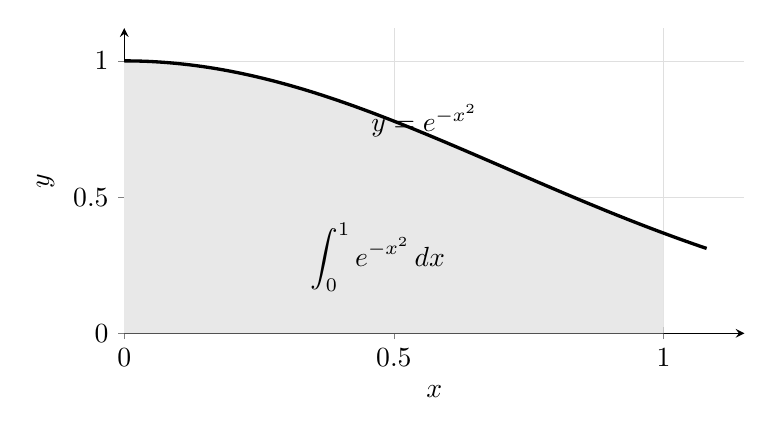
\begin{tikzpicture}
\begin{axis}[
    width=0.78\textwidth,
    height=0.45\textwidth,
    xmin=0, xmax=1.15,
    ymin=0, ymax=1.12,
    axis lines=left,
    xlabel={\(x\)},
    ylabel={\(y\)},
    xtick={0,0.5,1},
    ytick={0,0.5,1},
    grid=both,
    grid style={line width=.1pt, draw=gray!25},
]
\addplot[domain=0:1, samples=150, fill=gray!18, draw=none] {exp(-x^2)} \closedcycle;
\addplot[very thick, domain=0:1.08, samples=150] {exp(-x^2)};
\node[anchor=west] at (axis cs:0.44,0.78) {\(y=e^{-x^2}\)};
\node at (axis cs:0.47,0.28) {\(\displaystyle \int_0^1 e^{-x^2}\,dx\)};
\end{axis}
\end{tikzpicture}
\caption{The area \(\int_0^1 e^{-x^2}\,dx\) exists, even though the antiderivative is not elementary.}
\label{fig:gaussian-integral-piece}
\end{figure}

The difficulty is not the integral.  The difficulty is the antiderivative.  There is no
elementary function \(F\) such that

\[
F'(x)=e^{-x^2}.
\]

Proving that fact belongs to a later course.  For us, the practical consequence is enough:
the Fundamental Theorem cannot turn this integral into a simple endpoint calculation
using familiar functions.

But the integral still has a decimal value.  In fact,

\[
\int_0^1 e^{-x^2}\,dx\approx 0.746824.
\]

A numerical method should be able to recover this number, and should tell us how much
confidence to place in the digits.

\begin{quote}
\textbf{Important distinction.}

A function can be easy to evaluate but hard to antidifferentiate.

Numerical integration uses values of the function directly.  It does not require an
elementary antiderivative.
\end{quote}

\subsection{Speed versus accuracy}
\label{subsec:speed-versus-accuracy}

The original definition of the integral used Riemann sums:

\[
\sum_{j=1}^n f(x_j^*)\Delta x.
\]

If \(n\) is large and the function is well behaved, these sums can approximate the
integral well.  But a large \(n\) means many function evaluations.

There is a practical tradeoff:

\[
\text{more samples}
\quad\Longrightarrow\quad
\text{usually better accuracy, but more computation}.
\]

The word ``usually'' matters.  More samples help when they are used intelligently and
when the function is well behaved on the interval.  They do not automatically fix every
problem.

For example, if the integrand has a sharp spike, a coarse grid may miss it.  If the
integral is improper, applying a rule directly at an infinite endpoint or a vertical
asymptote may make no sense.  If a computer subtracts nearly equal numbers many
times, roundoff error may accumulate.

So numerical integration has two parts:

\[
\text{choose a reasonable approximation rule}
\]

and

\[
\text{estimate or control the error}.
\]

A fast approximation without an error estimate is only a guess with arithmetic attached.

\subsection{The role of error estimates}
\label{subsec:role-of-error-estimates}

Let

\[
I=\int_a^b f(x)\,dx
\]

be the exact value of an integral, and let \(A\) be an approximation.

The \emph{absolute error} is

\[
\boxed{
|I-A|.
}
\]

If

\[
|I-A|<0.001,
\]

then the approximation is within \(0.001\) of the true value.

Sometimes we care about the size of the error relative to the size of the true answer.  If
\(I\neq0\), the \emph{relative error} is

\[
\boxed{
\frac{|I-A|}{|I|}.
}
\]

For example, an absolute error of \(0.01\) is large if the true value is \(0.02\), but tiny if
the true value is \(10{,}000\).

\begin{quote}
\textbf{Numerical integration needs an error statement.}

A useful numerical answer should say something like

\[
\int_a^b f(x)\,dx\approx A
\]

with

\[
|I-A|<\text{known tolerance}.
\]
\end{quote}

There are two common ways to judge an approximation.

First, if we know enough about the function, we can use an \emph{error bound}.  An error
bound gives a guaranteed maximum possible error.

Second, if we compute several approximations using smaller and smaller step sizes, we
can watch the values stabilize.  This gives evidence, and often very good evidence, but it
is not the same as a proof unless it is supported by a theorem.

\paragraph{Example: watching approximations stabilize.}
For

\[
I=\int_0^1 e^{-x^2}\,dx,
\]

a numerical computation might produce the following approximations.

\begin{center}
\begin{tabular}{c|c}
\textbf{number of subintervals} & \textbf{approximation} \\ \hline
\(4\) & \(0.748747\) \\
\(8\) & \(0.747290\) \\
\(16\) & \(0.746941\) \\
\(32\) & \(0.746853\)
\end{tabular}
\end{center}

The values appear to be approaching a number near

\[
0.7468.
\]

That is encouraging.  But the table alone does not prove how close the last value is.
For proof, we need an error estimate.

The next section builds two rules whose geometry is easy to see and whose errors can be
controlled: the midpoint rule and the trapezoidal rule.

\section{Midpoint and trapezoidal rules}
\label{sec:midpoint-trapezoidal-rules}

A rectangle is the simplest approximation to area.  But there is more than one sensible
rectangle, and a rectangle is not the only simple shape.

On a short interval \([a,b]\), the graph may not be exactly straight, but it may be close to
straight.  This suggests two improvements over the roughest left and right rectangle
rules:

\[
\text{use the value at the midpoint}
\]

or

\[
\text{connect the endpoint values by a straight line}.
\]

These ideas give the midpoint rule and the trapezoidal rule.

\subsection{Geometry of the midpoint rule}
\label{subsec:geometry-midpoint-rule}

On a single interval \([a,b]\), the midpoint is

\[
m=\frac{a+b}{2}.
\]

The midpoint rule approximates the integral by a rectangle whose height is the function
value at the midpoint:

\[
\boxed{
\int_a^b f(x)\,dx\approx (b-a)f\left(\frac{a+b}{2}\right).
}
\]

The area of the rectangle is

\[
\text{width}\cdot\text{midpoint height}.
\]

\begin{figure}[h]
\centering
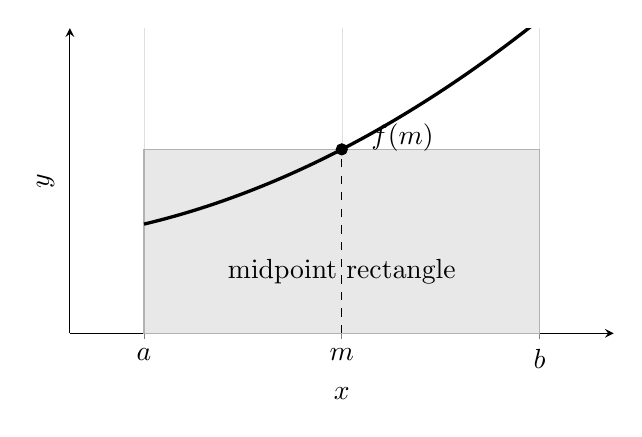
\begin{tikzpicture}
\begin{axis}[
    width=0.70\textwidth,
    height=0.45\textwidth,
    xmin=0, xmax=2.2,
    ymin=0, ymax=3.2,
    axis lines=left,
    xlabel={\(x\)},
    ylabel={\(y\)},
    xtick={0.3,1.1,1.9},
    xticklabels={\(a\),\(m\),\(b\)},
    ytick=\empty,
    grid=both,
    grid style={line width=.1pt, draw=gray!25},
]
\draw[fill=gray!18, draw=gray!60]
  (axis cs:0.3,0) rectangle (axis cs:1.9,{1+0.35*1.1+0.45*1.1^2});
\addplot[very thick, domain=0.3:1.9, samples=120] {1+0.35*x+0.45*x^2};
\addplot[only marks, mark=*] coordinates {(1.1,{1+0.35*1.1+0.45*1.1^2})};
\draw[dashed] (axis cs:1.1,0) -- (axis cs:1.1,{1+0.35*1.1+0.45*1.1^2});
\node[anchor=west] at (axis cs:1.18,2.05) {\(f(m)\)};
\node at (axis cs:1.1,0.65) {midpoint rectangle};
\end{axis}
\end{tikzpicture}
\caption{The midpoint rule uses one rectangle whose height is taken at the midpoint.}
\label{fig:midpoint-single-interval}
\end{figure}

Why use the midpoint instead of an endpoint?  The midpoint balances the interval.  If the
function is increasing, a left rectangle underestimates and a right rectangle overestimates.
The midpoint often cancels part of those errors.

For a line, the cancellation is perfect.

\paragraph{Example: midpoint rule is exact for a line.}
Let

\[
f(x)=2x+1
\]

on \([0,4]\).  The exact integral is

\[
\int_0^4 (2x+1)\,dx
=
\left(x^2+x\right)\Big|_0^4
=
20.
\]

The midpoint is

\[
m=2.
\]

The midpoint rectangle gives

\[
(4-0)f(2)=4(5)=20.
\]

So the midpoint rule gives the exact answer.

This happens for every linear function on every interval.  The midpoint height of a line
is exactly the average height of the line.

\subsection{Geometry of the trapezoidal rule}
\label{subsec:geometry-trapezoidal-rule}

The trapezoidal rule uses both endpoint values.  It connects

\[
(a,f(a))
\qquad\text{and}\qquad
(b,f(b))
\]

by a straight line, then takes the area under that line.

The resulting shape is a trapezoid with parallel vertical sides of heights \(f(a)\) and
\(f(b)\), and width \(b-a\).  Its area is

\[
\text{width}\cdot\text{average of the two heights}.
\]

Thus

\[
\boxed{
\int_a^b f(x)\,dx\approx
\frac{b-a}{2}\bigl(f(a)+f(b)\bigr).
}
\]

\begin{figure}[h]
\centering
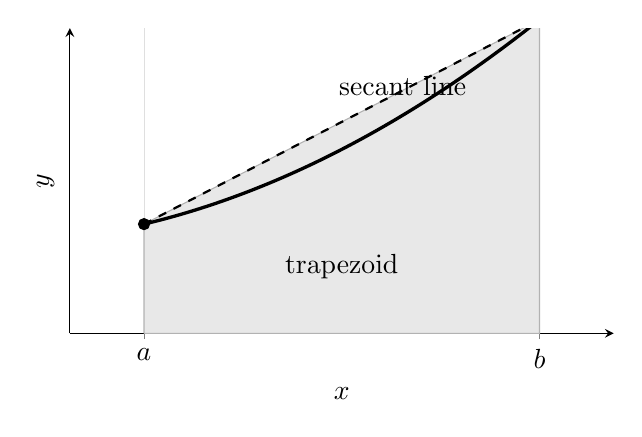
\begin{tikzpicture}
\begin{axis}[
    width=0.70\textwidth,
    height=0.45\textwidth,
    xmin=0, xmax=2.2,
    ymin=0, ymax=3.2,
    axis lines=left,
    xlabel={\(x\)},
    ylabel={\(y\)},
    xtick={0.3,1.9},
    xticklabels={\(a\),\(b\)},
    ytick=\empty,
    grid=both,
    grid style={line width=.1pt, draw=gray!25},
]
\addplot[fill=gray!18, draw=gray!60] coordinates {
  (0.3,0)
  (0.3,{1+0.35*0.3+0.45*0.3^2})
  (1.9,{1+0.35*1.9+0.45*1.9^2})
  (1.9,0)
  (0.3,0)
};
\addplot[very thick, domain=0.3:1.9, samples=120] {1+0.35*x+0.45*x^2};
\addplot[thick, dashed] coordinates {
  (0.3,{1+0.35*0.3+0.45*0.3^2})
  (1.9,{1+0.35*1.9+0.45*1.9^2})
};
\addplot[only marks, mark=*] coordinates {
  (0.3,{1+0.35*0.3+0.45*0.3^2})
  (1.9,{1+0.35*1.9+0.45*1.9^2})
};
\node at (axis cs:1.1,0.70) {trapezoid};
\node[anchor=west] at (axis cs:1.05,2.6) {secant line};
\end{axis}
\end{tikzpicture}
\caption{The trapezoidal rule replaces the graph by the secant line over the interval.}
\label{fig:trapezoid-single-interval}
\end{figure}

The trapezoidal rule is also exact for a line, because the secant line is the graph itself.

\subsection{Composite rules}
\label{subsec:composite-midpoint-trapezoidal-rules}

One wide rectangle or one wide trapezoid is usually too crude.  The remedy is to divide
the interval into smaller pieces and apply the rule on each piece.

Divide \([a,b]\) into \(n\) equal subintervals.  Let

\[
\Delta x=\frac{b-a}{n},
\]

and define the grid points

\[
x_0=a,\qquad x_1=a+\Delta x,\qquad x_2=a+2\Delta x,\qquad \ldots,\qquad x_n=b.
\]

The midpoint of the \(i\)th subinterval \([x_{i-1},x_i]\) is

\[
\overline{x}_i=\frac{x_{i-1}+x_i}{2}.
\]

\begin{quote}
\textbf{Composite midpoint rule.}

\[
\boxed{
M_n=\Delta x\sum_{i=1}^n f(\overline{x}_i).
}
\]

Here \(M_n\) approximates

\[
\int_a^b f(x)\,dx.
\]
\end{quote}

The trapezoidal rule gives one trapezoid on each subinterval.  The endpoint values inside
the interval are used twice, once from the left trapezoid and once from the right
trapezoid.  That is why the interior values receive full weight, while the two outer
endpoint values receive half weight.

\begin{quote}
\textbf{Composite trapezoidal rule.}

\[
\boxed{
T_n=
\Delta x\left[
\frac12 f(x_0)+f(x_1)+f(x_2)+\cdots+f(x_{n-1})+\frac12 f(x_n)
\right].
}
\]

Here \(T_n\) approximates

\[
\int_a^b f(x)\,dx.
\]
\end{quote}

\begin{figure}[h]
\centering
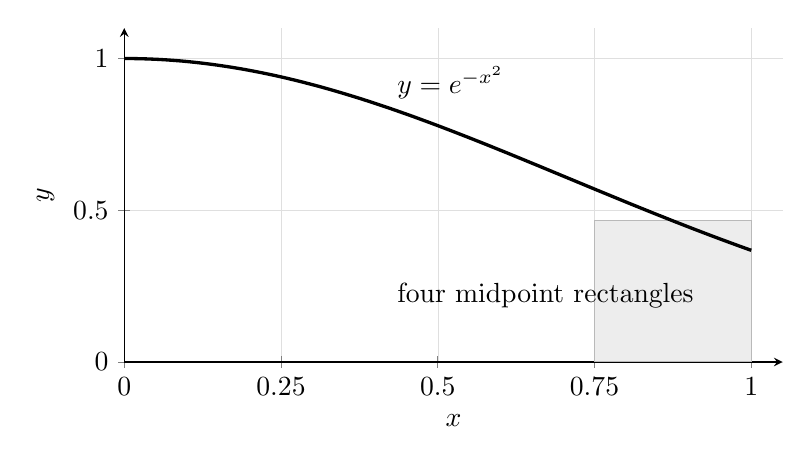
\begin{tikzpicture}
\begin{axis}[
    width=0.82\textwidth,
    height=0.48\textwidth,
    xmin=0, xmax=1.05,
    ymin=0, ymax=1.1,
    axis lines=left,
    xlabel={\(x\)},
    ylabel={\(y\)},
    xtick={0,0.25,0.5,0.75,1},
    ytick={0,0.5,1},
    grid=both,
    grid style={line width=.1pt, draw=gray!25},
]
% midpoint rectangles for exp(-x^2) on [0,1], n=4
\pgfplotsinvokeforeach{0,1,2,3}{
  \pgfmathsetmacro{\left}{0.25*#1}
  \pgfmathsetmacro{\right}{0.25*(#1+1)}
  \pgfmathsetmacro{\mid}{0.25*(#1+0.5)}
  \pgfmathsetmacro{\height}{exp(-\mid*\mid)}
  \draw[fill=gray!14, draw=gray!55]
    (axis cs:\left,0) rectangle (axis cs:\right,\height);
}
\addplot[very thick, domain=0:1, samples=150] {exp(-x^2)};
\node[anchor=west] at (axis cs:0.42,0.92) {\(y=e^{-x^2}\)};
\node[anchor=west] at (axis cs:0.42,0.22) {four midpoint rectangles};
\end{axis}
\end{tikzpicture}
\caption{The composite midpoint rule adds midpoint rectangles over smaller subintervals.}
\label{fig:composite-midpoint-exp}
\end{figure}

\subsection{Example: approximating a non-elementary integral}
\label{subsec:example-approx-e-minus-x-squared}

Approximate

\[
I=\int_0^1 e^{-x^2}\,dx
\]

using \(n=4\) subintervals.

Here

\[
\Delta x=\frac{1-0}{4}=\frac14.
\]

The grid points are

\[
0,\quad 0.25,\quad 0.50,\quad 0.75,\quad 1.00.
\]

The midpoint values are taken at

\[
0.125,\quad 0.375,\quad 0.625,\quad 0.875.
\]

The needed function values are:

\begin{center}
\begin{tabular}{c|c|c|c}
\textbf{subinterval} & \(\overline{x}_i\) & \(f(\overline{x}_i)\) & \textbf{endpoint values for trapezoids} \\ \hline
\([0,0.25]\) & \(0.125\) & \(0.984496\) & \(f(0)=1.000000,\ f(0.25)=0.939413\) \\
\([0.25,0.50]\) & \(0.375\) & \(0.868815\) & \(f(0.25)=0.939413,\ f(0.50)=0.778801\) \\
\([0.50,0.75]\) & \(0.625\) & \(0.676634\) & \(f(0.50)=0.778801,\ f(0.75)=0.569783\) \\
\([0.75,1.00]\) & \(0.875\) & \(0.465043\) & \(f(0.75)=0.569783,\ f(1)=0.367879\)
\end{tabular}
\end{center}

The midpoint approximation is

\[
M_4
=
\frac14
\left(
0.984496+0.868815+0.676634+0.465043
\right).
\]

So

\[
\boxed{
M_4\approx 0.748747.
}
\]

The trapezoidal approximation is

\[
T_4
=
\frac14
\left[
\frac12(1.000000)
+0.939413+0.778801+0.569783
+\frac12(0.367879)
\right].
\]

Thus

\[
\boxed{
T_4\approx 0.742984.
}
\]

A more accurate value is

\[
I\approx 0.746824.
\]

So in this example, with \(n=4\),

\[
T_4<I<M_4.
\]

This straddling is useful, but it is not guaranteed for every function.  To understand when
an approximation is above or below the true value, we need to look at concavity.

\subsection{Error patterns from concavity}
\label{subsec:error-patterns-from-concavity}

The trapezoidal rule replaces the graph by a secant line.  The midpoint rule replaces the
graph by a horizontal line at the midpoint height.

Concavity tells us which approximation lies above or below the true area.

If

\[
f''(x)>0
\]

on an interval, the graph is concave up.  It bends upward.  The secant line lies above the
graph, so the trapezoid overestimates the integral.

For the same concave-up graph, the midpoint rectangle underestimates the integral.  The
curve spends more area above the midpoint height than below it.

\paragraph{Example: concave up.}
Let

\[
f(x)=x^2
\]

on \([0,1]\).  The exact value is

\[
I=\int_0^1 x^2\,dx=\frac13.
\]

With one trapezoid,

\[
T_1=\frac12(f(0)+f(1))=\frac12.
\]

With one midpoint rectangle,

\[
M_1=f\left(\frac12\right)=\frac14.
\]

So

\[
M_1<I<T_1.
\]

The graph is concave up, and the error signs match the picture.

If

\[
f''(x)<0
\]

on an interval, the graph is concave down.  The pattern reverses:

\[
T_n<I<M_n
\]

when the concavity stays down on the whole interval.

\paragraph{Example: concave down.}
Let

\[
f(x)=1-x^2
\]

on \([0,1]\).  Then

\[
I=\int_0^1 (1-x^2)\,dx=\frac23.
\]

With one trapezoid,

\[
T_1=\frac12(f(0)+f(1))=\frac12.
\]

With one midpoint rectangle,

\[
M_1=f\left(\frac12\right)=\frac34.
\]

Thus

\[
T_1<I<M_1.
\]

\begin{figure}[h]
\centering
\begin{minipage}{0.47\textwidth}
\centering
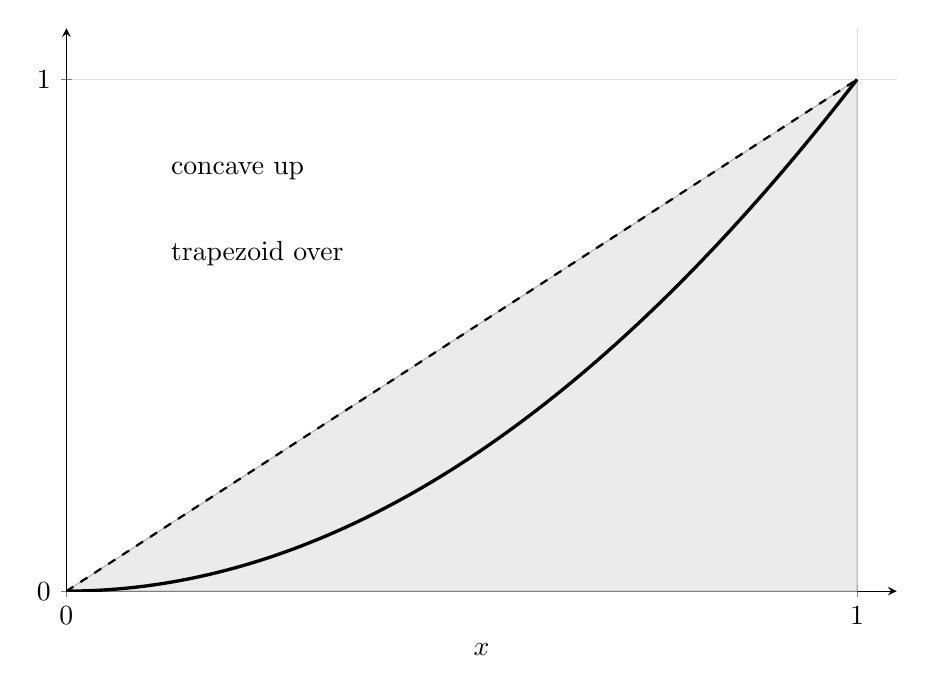
\begin{tikzpicture}
\begin{axis}[
    width=\textwidth,
    height=0.72\textwidth,
    xmin=0, xmax=1.05,
    ymin=0, ymax=1.1,
    axis lines=left,
    xlabel={\(x\)},
    ylabel={},
    xtick={0,1},
    ytick={0,1},
    grid=both,
    grid style={line width=.1pt, draw=gray!25},
]
\addplot[fill=gray!16, draw=gray!60] coordinates {(0,0) (0,0) (1,1) (1,0) (0,0)};
\addplot[very thick, domain=0:1, samples=120] {x^2};
\addplot[thick, dashed] coordinates {(0,0) (1,1)};
\node[anchor=west] at (axis cs:0.12,0.82) {concave up};
\node[anchor=west] at (axis cs:0.12,0.66) {trapezoid over};
\end{axis}
\end{tikzpicture}
\end{minipage}
\hfill
\begin{minipage}{0.47\textwidth}
\centering
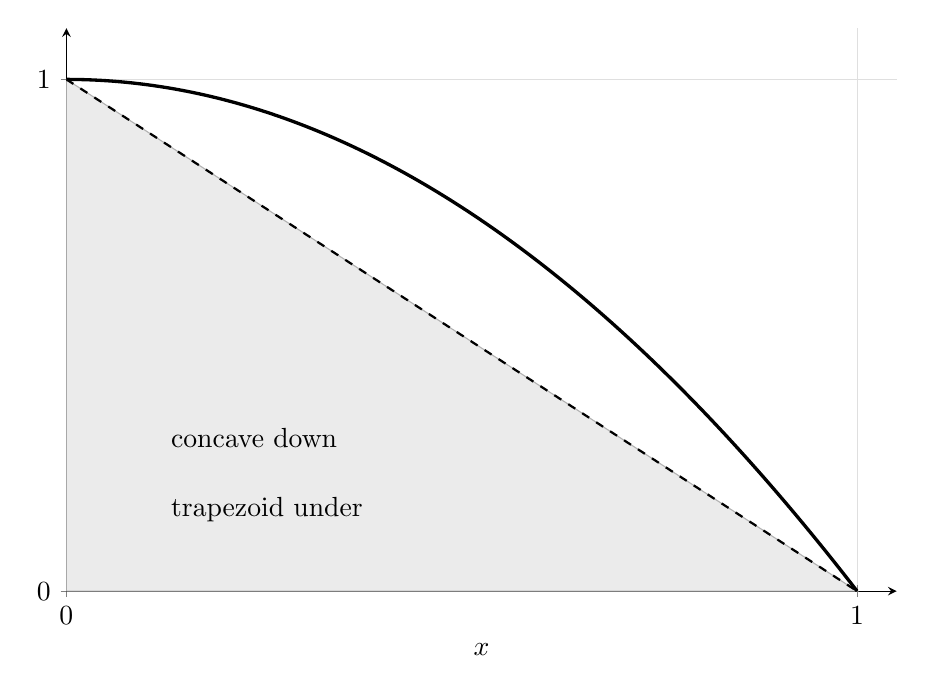
\begin{tikzpicture}
\begin{axis}[
    width=\textwidth,
    height=0.72\textwidth,
    xmin=0, xmax=1.05,
    ymin=0, ymax=1.1,
    axis lines=left,
    xlabel={\(x\)},
    ylabel={},
    xtick={0,1},
    ytick={0,1},
    grid=both,
    grid style={line width=.1pt, draw=gray!25},
]
\addplot[fill=gray!16, draw=gray!60] coordinates {(0,0) (0,1) (1,0) (1,0) (0,0)};
\addplot[very thick, domain=0:1, samples=120] {1-x^2};
\addplot[thick, dashed] coordinates {(0,1) (1,0)};
\node[anchor=west] at (axis cs:0.12,0.30) {concave down};
\node[anchor=west] at (axis cs:0.12,0.16) {trapezoid under};
\end{axis}
\end{tikzpicture}
\end{minipage}
\caption{For concave-up graphs, trapezoids lie above the curve.  For concave-down graphs, trapezoids lie below.}
\label{fig:trapezoid-concavity-error}
\end{figure}

\begin{quote}
\textbf{Concavity error pattern.}

Assume \(f\) is twice differentiable and the concavity does not change on \([a,b]\).

\begin{center}
\begin{tabular}{c|c|c}
\textbf{shape} & \textbf{trapezoidal rule} & \textbf{midpoint rule} \\ \hline
\(f''>0\), concave up & overestimates & underestimates \\[3pt]
\(f''<0\), concave down & underestimates & overestimates
\end{tabular}
\end{center}
\end{quote}

\paragraph{Warning: changing concavity.}
If the function changes concavity on the interval, these simple over-under rules may not
apply to the whole interval.

For example,

\[
f(x)=e^{-x^2}
\]

has

\[
f''(x)=(4x^2-2)e^{-x^2}.
\]

This changes sign at

\[
x=\frac{1}{\sqrt2}.
\]

So on \([0,1]\), the graph is concave down at first and concave up later.  We should not
expect one global concavity picture to explain all of the error.

In that case, use error bounds.

\subsection{Error bounds}
\label{subsec:midpoint-trapezoid-error-bounds}

An error pattern tells us the direction of the error.  An error bound tells us how large the
error can be.

The size of the error is controlled by curvature.  If the graph is nearly linear on each
small interval, the midpoint and trapezoidal rules are accurate.  The second derivative
measures how far the graph is from being linear.

\begin{quote}
\textbf{Error bounds for the composite midpoint and trapezoidal rules.}

Suppose \(f''\) is continuous on \([a,b]\), and suppose

\[
|f''(x)|\le K
\]

for all \(x\in[a,b]\).

Let

\[
I=\int_a^b f(x)\,dx.
\]

If \(M_n\) is the composite midpoint approximation using \(n\) equal subintervals, then

\[
\boxed{
|I-M_n|\le \frac{K(b-a)^3}{24n^2}.
}
\]

If \(T_n\) is the composite trapezoidal approximation using \(n\) equal subintervals, then

\[
\boxed{
|I-T_n|\le \frac{K(b-a)^3}{12n^2}.
}
\]
\end{quote}

The important feature is the factor

\[
\frac{1}{n^2}.
\]

Doubling the number of subintervals usually divides these error bounds by about \(4\).

The midpoint bound is half the trapezoidal bound when the same \(K\), \(a\), \(b\), and
\(n\) are used.  This does not mean the midpoint rule is always exactly twice as accurate,
but it explains why midpoint approximations often perform very well.

\paragraph{Idea of the proof.}
On one short subinterval of width \(\Delta x\), Taylor's theorem says that the failure of
the graph to be linear is controlled by \(f''\).  The one-interval trapezoid error is at most

\[
\frac{K(\Delta x)^3}{12},
\]

and the one-interval midpoint error is at most

\[
\frac{K(\Delta x)^3}{24}.
\]

There are \(n\) subintervals, and

\[
\Delta x=\frac{b-a}{n}.
\]

Adding the one-interval bounds gives

\[
n\cdot \frac{K(\Delta x)^3}{12}
=
n\cdot \frac{K}{12}\left(\frac{b-a}{n}\right)^3
=
\frac{K(b-a)^3}{12n^2}
\]

for the trapezoidal rule.  The midpoint calculation is the same, with \(24\) in place of
\(12\).

The constants come from integrating the quadratic error term in Taylor's formula.

\paragraph{Example: how many subintervals are enough?}
Use the midpoint rule to approximate

\[
\int_0^1 e^{-x^2}\,dx
\]

with error less than

\[
0.0005.
\]

For

\[
f(x)=e^{-x^2},
\]

we computed

\[
f''(x)=(4x^2-2)e^{-x^2}.
\]

On \([0,1]\), a simple bound is

\[
|f''(x)|\le 2.
\]

So we may take

\[
K=2.
\]

The midpoint error bound gives

\[
|I-M_n|
\le
\frac{K(b-a)^3}{24n^2}
=
\frac{2(1)^3}{24n^2}
=
\frac{1}{12n^2}.
\]

We want

\[
\frac{1}{12n^2}<0.0005.
\]

This is equivalent to

\[
12n^2>2000,
\]

so

\[
n^2>\frac{2000}{12}\approx 166.67.
\]

Thus

\[
n>12.91.
\]

Therefore

\[
\boxed{
n=13
}
\]

subintervals are enough to guarantee midpoint error less than \(0.0005\).

The actual error may be smaller.  The bound is a guarantee, not a prediction of the exact
error.

\paragraph{Why the hypotheses matter.}
The error bounds above assume that \(f''\) is continuous and bounded on \([a,b]\).  If
that fails, the formulas may not apply.

For example,

\[
f(x)=\sqrt{x}
\]

is continuous on \([0,1]\), and the integral

\[
\int_0^1 \sqrt{x}\,dx
\]

exists.  But

\[
f''(x)=-\frac{1}{4x^{3/2}}
\]

for \(x>0\), and this becomes unbounded as \(x\to0^+\).

The midpoint and trapezoidal rules can still be used to approximate the integral, but the
standard \(K\)-bound above cannot be used on \([0,1]\), because there is no finite number
\(K\) with

\[
|f''(x)|\le K
\]

on the whole interval.

\begin{quote}
\textbf{Warning.}
A numerical rule may still produce numbers when its error-bound hypotheses fail.

The formula for the guarantee is what fails, not necessarily the approximation itself.
\end{quote}

This warning matters in applications.  Before using an error bound, check the interval,
the continuity of the derivatives, and whether the integral is proper.

The midpoint and trapezoidal rules approximate a curve by flat or straight pieces.  The
next rule asks a natural question:

\[
\boxed{
\text{What if we approximate the graph by a parabola instead?}
}
\]

That idea leads to Simpson's Rule.
\section{Simpson's Rule}
\label{sec:simpsons-rule}

The midpoint and trapezoidal rules replaced the graph by something simple: a
horizontal line or a straight line.  Those approximations are easy to compute, and
their errors are controlled by curvature.

But a curve is not usually straight.  On a short interval, a better first picture may be a
parabola.

That is the idea behind Simpson's Rule.

\[
\boxed{
\text{Use a quadratic curve instead of a line.}
}
\]

The reward is surprisingly large.  Midpoint and trapezoidal errors usually shrink like
\(1/n^2\).  Simpson's Rule, for smooth functions, usually shrinks like \(1/n^4\).

\subsection{Quadratic approximation on pairs of intervals}
\label{subsec:quadratic-approximation-pairs-intervals}

A line is determined by two points.  A parabola is determined by three points.

So Simpson's Rule uses three equally spaced sample points:

\[
x_0,\qquad x_1,\qquad x_2,
\]

where

\[
x_1=x_0+\Delta x,
\qquad
x_2=x_0+2\Delta x.
\]

The middle point \(x_1\) is the midpoint of \([x_0,x_2]\).

The function values are

\[
f(x_0),\qquad f(x_1),\qquad f(x_2).
\]

Through the three points

\[
(x_0,f(x_0)),\qquad (x_1,f(x_1)),\qquad (x_2,f(x_2)),
\]

there is exactly one quadratic polynomial.  Simpson's Rule integrates that quadratic
instead of the original function.

\begin{figure}[h]
\centering
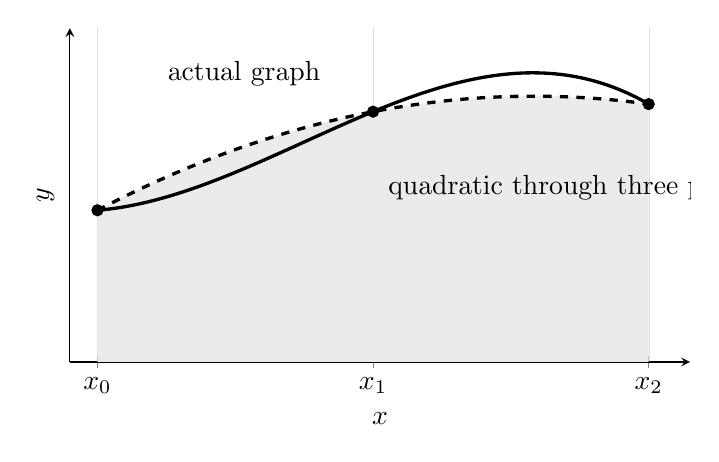
\begin{tikzpicture}
\begin{axis}[
    width=0.78\textwidth,
    height=0.48\textwidth,
    xmin=-0.1, xmax=2.15,
    ymin=0, ymax=2.2,
    axis lines=left,
    xlabel={\(x\)},
    ylabel={\(y\)},
    xtick={0,1,2},
    xticklabels={\(x_0\),\(x_1\),\(x_2\)},
    ytick=\empty,
    grid=both,
    grid style={line width=.1pt, draw=gray!25},
]
% Quadratic fill/interpolant
\addplot[domain=0:2, samples=100, fill=gray!16, draw=none] {1+0.95*x-0.3*x^2} \closedcycle;
\addplot[very thick, dashed, domain=0:2, samples=100] {1+0.95*x-0.3*x^2};

% A nearby non-quadratic function with same values at 0,1,2
\addplot[very thick, domain=0:2, samples=150] {1+0.15*x+0.9*x^2-0.4*x^3};

\addplot[only marks, mark=*] coordinates {
    (0,1)
    (1,1.65)
    (2,1.70)
};

\node[anchor=west] at (axis cs:0.22,1.9) {actual graph};
\node[anchor=west] at (axis cs:1.02,1.15) {quadratic through three points};
\end{axis}
\end{tikzpicture}
\caption{Simpson's Rule replaces the graph on two subintervals by the parabola through three sample points.}
\label{fig:simpson-quadratic-through-three-points}
\end{figure}

The formula is simple:

\[
\boxed{
\int_{x_0}^{x_2} f(x)\,dx
\approx
\frac{\Delta x}{3}
\left[
f(x_0)+4f(x_1)+f(x_2)
\right].
}
\]

The middle value receives weight \(4\).  The endpoint values receive weight \(1\).

\paragraph{Where the weights come from.}
To see the weights, shift and scale the interval so that the three sample points become

\[
-1,\qquad 0,\qquad 1.
\]

Let

\[
p(u)=Au^2+Bu+C
\]

be the quadratic through

\[
(-1,y_0),\qquad (0,y_1),\qquad (1,y_2).
\]

Then

\[
p(0)=C=y_1.
\]

Also

\[
p(-1)=A-B+C=y_0,
\]

and

\[
p(1)=A+B+C=y_2.
\]

Adding these last two equations gives

\[
2A+2C=y_0+y_2.
\]

Since \(C=y_1\),

\[
A=\frac{y_0+y_2-2y_1}{2}.
\]

Now integrate \(p\) from \(-1\) to \(1\):

\[
\int_{-1}^{1}p(u)\,du
=
\int_{-1}^{1}(Au^2+Bu+C)\,du.
\]

The odd term integrates to zero:

\[
\int_{-1}^{1}Bu\,du=0.
\]

So

\[
\int_{-1}^{1}p(u)\,du
=
A\int_{-1}^{1}u^2\,du+C\int_{-1}^{1}1\,du.
\]

Since

\[
\int_{-1}^{1}u^2\,du=\frac23
\]

and

\[
\int_{-1}^{1}1\,du=2,
\]

we get

\[
\int_{-1}^{1}p(u)\,du
=
\frac23A+2C.
\]

Substitute the values of \(A\) and \(C\):

\[
\frac23\cdot\frac{y_0+y_2-2y_1}{2}+2y_1
=
\frac13(y_0+y_2-2y_1)+2y_1.
\]

Therefore

\[
\int_{-1}^{1}p(u)\,du
=
\frac13(y_0+4y_1+y_2).
\]

Finally, returning to \(x\)-coordinates multiplies the integral by the spacing
\(\Delta x\).  Thus

\[
\int_{x_0}^{x_2}p(x)\,dx
=
\frac{\Delta x}{3}
\left[
y_0+4y_1+y_2
\right].
\]

That is Simpson's Rule.

\begin{quote}
\textbf{One-panel Simpson's Rule.}

If

\[
m=\frac{a+b}{2},
\]

then

\[
\boxed{
\int_a^b f(x)\,dx
\approx
\frac{b-a}{6}\left[
f(a)+4f(m)+f(b)
\right].
}
\]

This is the same formula as above, written for one interval \([a,b]\) with midpoint
\(m\).
\end{quote}

\paragraph{Example: exact for a quadratic.}
Use Simpson's Rule to compute

\[
\int_0^2 x^2\,dx.
\]

Here

\[
a=0,\qquad m=1,\qquad b=2.
\]

The Simpson approximation is

\[
\frac{2-0}{6}\left[f(0)+4f(1)+f(2)\right].
\]

Since \(f(x)=x^2\),

\[
f(0)=0,\qquad f(1)=1,\qquad f(2)=4.
\]

So

\[
S=\frac{2}{6}(0+4+4)=\frac{8}{3}.
\]

The exact value is

\[
\int_0^2 x^2\,dx
=
\left[\frac{x^3}{3}\right]_0^2
=
\frac83.
\]

So Simpson's Rule is exact in this example.

That should not be surprising.  Simpson's Rule integrates the quadratic interpolating
polynomial.  If the original function is already quadratic, the approximation is the
function itself.

\subsection{Composite Simpson's Rule}
\label{subsec:composite-simpsons-rule}

One parabola over a wide interval may not be enough.  As before, we divide the interval
into smaller pieces.

Let \([a,b]\) be divided into \(n\) equal subintervals, where \(n\) is even.  Define

\[
\Delta x=\frac{b-a}{n},
\]

and

\[
x_i=a+i\Delta x,
\qquad
i=0,1,2,\ldots,n.
\]

Because Simpson's Rule uses pairs of subintervals, \(n\) must be even.  We apply
Simpson's Rule on

\[
[x_0,x_2],\quad [x_2,x_4],\quad [x_4,x_6],\quad \ldots,\quad [x_{n-2},x_n].
\]

On the first pair,

\[
\int_{x_0}^{x_2} f(x)\,dx
\approx
\frac{\Delta x}{3}
\left[
f(x_0)+4f(x_1)+f(x_2)
\right].
\]

On the second pair,

\[
\int_{x_2}^{x_4} f(x)\,dx
\approx
\frac{\Delta x}{3}
\left[
f(x_2)+4f(x_3)+f(x_4)
\right].
\]

Adding the pieces, the shared endpoint values such as \(f(x_2)\) are counted twice.
That is why the even interior indices receive weight \(2\).

\begin{quote}
\textbf{Composite Simpson's Rule.}

Suppose \(n\) is even.  Then

\[
\boxed{
S_n=
\frac{\Delta x}{3}
\left[
f(x_0)
+4f(x_1)
+2f(x_2)
+4f(x_3)
+2f(x_4)
+\cdots
+4f(x_{n-1})
+f(x_n)
\right].
}
\]

The weights follow the pattern

\[
1,\ 4,\ 2,\ 4,\ 2,\ \ldots,\ 4,\ 1.
\]
\end{quote}

A compact way to remember the formula is:

\[
S_n
=
\frac{\Delta x}{3}
\left[
f(x_0)+f(x_n)
+
4\sum_{\substack{i=1\\ i\text{ odd}}}^{n-1} f(x_i)
+
2\sum_{\substack{i=2\\ i\text{ even}}}^{n-2} f(x_i)
\right].
\]

The odd interior points get weight \(4\).  The even interior points get weight \(2\).

\paragraph{Warning: \(n\) must be even.}
Composite Simpson's Rule pairs neighboring subintervals.  If \(n\) is odd, one
subinterval is left unpaired.

For example, \(n=5\) gives five subintervals.  Simpson's Rule can cover four of them
in two pairs, but one remains.  In that situation, either change \(n\) to an even number
or combine Simpson's Rule with another rule on the leftover interval.

For this course, when using Simpson's Rule, choose \(n\) even.

\subsection{Example: Simpson's Rule for \texorpdfstring{\(\int_0^1 e^{-x^2}\,dx\)}{int_0^1 e^{-x^2} dx}}
\label{subsec:simpson-example-e-minus-x-squared}

Approximate

\[
I=\int_0^1 e^{-x^2}\,dx
\]

using Simpson's Rule with \(n=4\).

Here

\[
\Delta x=\frac{1-0}{4}=\frac14.
\]

The grid points are

\[
x_0=0,\quad x_1=0.25,\quad x_2=0.50,\quad x_3=0.75,\quad x_4=1.
\]

The function values are:

\[
\begin{array}{c|ccccc}
x_i & 0 & 0.25 & 0.50 & 0.75 & 1.00 \\ \hline
e^{-x_i^2} & 1.000000 & 0.939413 & 0.778801 & 0.569783 & 0.367879
\end{array}
\]

Since \(n=4\), the weights are

\[
1,\ 4,\ 2,\ 4,\ 1.
\]

Therefore

\[
S_4
=
\frac{0.25}{3}
\left[
1.000000
+4(0.939413)
+2(0.778801)
+4(0.569783)
+0.367879
\right].
\]

Compute the weighted sum:

\[
1.000000
+3.757652
+1.557602
+2.279132
+0.367879
=
8.962265.
\]

Thus

\[
S_4=\frac{0.25}{3}(8.962265)\approx 0.746855.
\]

So

\[
\boxed{
\int_0^1 e^{-x^2}\,dx\approx 0.746855
}
\]

using Simpson's Rule with only four subintervals.

A more accurate value is

\[
0.746824\ldots,
\]

so this approximation is already quite good.

\begin{center}
\begin{tabular}{c|c}
\textbf{rule with \(n=4\)} & \textbf{approximation to \(\int_0^1 e^{-x^2}\,dx\)} \\ \hline
midpoint & \(0.748747\) \\
trapezoidal & \(0.742984\) \\
Simpson & \(0.746855\)
\end{tabular}
\end{center}

The Simpson value is much closer in this example.  The next subsection explains why
this often happens.

\subsection{Why Simpson's Rule is often much better}
\label{subsec:why-simpson-rule-better}

The midpoint and trapezoidal rules approximate a graph using degree \(0\) and degree
\(1\) shapes:

\[
\text{horizontal line},
\qquad
\text{straight line}.
\]

Simpson's Rule uses degree \(2\):

\[
\text{parabola}.
\]

So it should be exact for quadratic functions.  The surprise is that it is also exact for
cubic functions.

To see why, work on the symmetric interval \([-1,1]\).  Simpson's Rule says

\[
\int_{-1}^{1} f(x)\,dx
\approx
\frac13\left[f(-1)+4f(0)+f(1)\right].
\]

Check the four basic powers \(1,x,x^2,x^3\).

For \(f(x)=1\),

\[
\int_{-1}^{1}1\,dx=2,
\]

and Simpson gives

\[
\frac13(1+4+1)=2.
\]

For \(f(x)=x\),

\[
\int_{-1}^{1}x\,dx=0,
\]

and Simpson gives

\[
\frac13(-1+0+1)=0.
\]

For \(f(x)=x^2\),

\[
\int_{-1}^{1}x^2\,dx=\frac23,
\]

and Simpson gives

\[
\frac13(1+0+1)=\frac23.
\]

For \(f(x)=x^3\),

\[
\int_{-1}^{1}x^3\,dx=0,
\]

and Simpson gives

\[
\frac13(-1+0+1)=0.
\]

So Simpson's Rule is exact for all polynomials of degree at most \(3\).  Any cubic is a
linear combination of

\[
1,\quad x,\quad x^2,\quad x^3.
\]

Since both integration and Simpson's formula are linear, exactness for these four
powers gives exactness for every cubic.

\begin{quote}
\textbf{Key fact.}
Simpson's Rule is built from a quadratic approximation, but it integrates every cubic
polynomial exactly.
\end{quote}

This is why Simpson's Rule can outperform what its construction suggests.

There is also a useful geometric way to remember the improvement.  On a concave-up
graph, the trapezoidal rule tends to overestimate and the midpoint rule tends to
underestimate.  Simpson's Rule is the weighted average

\[
\boxed{
S=\frac13T+\frac23M
}
\]

on a single interval, where \(T\) is the one-trapezoid approximation and \(M\) is the
midpoint approximation.

Indeed,

\[
T=\frac{b-a}{2}\bigl(f(a)+f(b)\bigr),
\]

and

\[
M=(b-a)f(m).
\]

Then

\[
\frac13T+\frac23M
=
\frac{b-a}{6}\bigl(f(a)+f(b)\bigr)
+
\frac{2(b-a)}{3}f(m).
\]

So

\[
\frac13T+\frac23M
=
\frac{b-a}{6}
\left[
f(a)+4f(m)+f(b)
\right],
\]

which is Simpson's Rule.

The leading curvature errors of \(T\) and \(M\) have opposite signs.  Simpson's Rule
combines them in just the right proportion to cancel much of that error.

\subsection{Simpson error bound}
\label{subsec:simpson-error-bound}

The midpoint and trapezoidal error bounds were controlled by \(f''\), because lines
fail when curvature is present.

Simpson's Rule is exact for cubics.  So its first possible error comes from behavior
beyond cubic.  That is why the fourth derivative appears.

\begin{quote}
\textbf{Error bound for composite Simpson's Rule.}

Suppose \(f^{(4)}\) is continuous on \([a,b]\), and suppose

\[
|f^{(4)}(x)|\le K
\]

for all \(x\in[a,b]\).

Let \(S_n\) be the composite Simpson approximation using \(n\) equal subintervals,
where \(n\) is even.  Then

\[
\boxed{
\left|
\int_a^b f(x)\,dx-S_n
\right|
\le
\frac{K(b-a)^5}{180n^4}.
}
\]
\end{quote}

The important feature is

\[
\frac{1}{n^4}.
\]

Doubling \(n\) divides the error bound by

\[
2^4=16.
\]

That is a much faster improvement than the \(1/n^2\) behavior of the midpoint and
trapezoidal rules.

\paragraph{Example: a guaranteed Simpson approximation.}
Use Simpson's Rule to approximate

\[
\int_0^1 e^{-x^2}\,dx
\]

with guaranteed error less than \(0.0005\).

For

\[
f(x)=e^{-x^2},
\]

a calculation gives

\[
f^{(4)}(x)=\left(16x^4-48x^2+12\right)e^{-x^2}.
\]

On \([0,1]\), a derivative check shows

\[
|f^{(4)}(x)|\le 12.
\]

So we may take

\[
K=12.
\]

The Simpson error bound gives

\[
|I-S_n|
\le
\frac{12(1)^5}{180n^4}
=
\frac{1}{15n^4}.
\]

We want

\[
\frac{1}{15n^4}<0.0005.
\]

This is equivalent to

\[
15n^4>2000,
\]

or

\[
n^4>\frac{2000}{15}\approx 133.33.
\]

Taking fourth roots,

\[
n>3.40.
\]

Since Simpson's Rule requires \(n\) even, we take

\[
\boxed{n=4.}
\]

So \(4\) subintervals are enough to guarantee error less than \(0.0005\).

With \(n=4\), we found

\[
S_4\approx0.746855.
\]

The actual error is even smaller than the guaranteed bound.

\begin{quote}
\textbf{A bound is a guarantee, not a prediction.}

An error bound tells us the approximation cannot be worse than a certain amount.
It does not usually tell us the actual error exactly.
\end{quote}

\paragraph{Why the hypotheses matter.}
The Simpson error bound assumes that \(f^{(4)}\) exists, is continuous, and is bounded
on the interval.

For example,

\[
f(x)=\sqrt{x}
\]

is continuous on \([0,1]\), and the integral

\[
\int_0^1 \sqrt{x}\,dx
\]

exists.  But the derivatives of \(f\) become singular near \(x=0\).  In particular, the
fourth derivative is unbounded near \(0\).

Simpson's Rule may still produce useful approximations, but the standard Simpson
error bound does not apply on \([0,1]\).

\[
\boxed{
\text{The numerical rule can still be used.  The guarantee is what fails.}
}
\]

That warning is important in computation.  A formula can return a number even when
the theorem that estimates its error does not apply.

Numerical integration approximates accumulation.  But the other half of calculus can
also be approximated.  If we know values of a function from data, can we estimate its
derivative?

That question leads to numerical differentiation.

\section{Numerical differentiation}
\label{sec:numerical-differentiation}

Integration is forgiving.  It averages values over an interval.

Differentiation is less forgiving.  It subtracts nearby values and divides by a small
number.

That difference matters.

If we know a formula for \(f\), exact differentiation may be best.  But in experiments,
we may only know values from a table.  A motion sensor records position.  A weather
station records temperature.  A lab instrument records concentration.  We then ask:

\[
\boxed{
\text{Can we estimate the instantaneous rate of change from sampled values?}
}
\]

The answer is yes, but with a warning: smaller steps are not always better.

\subsection{Forward, backward, and centered differences}
\label{subsec:forward-backward-centered-differences}

The derivative at \(a\) is

\[
f'(a)=\lim_{h\to0}\frac{f(a+h)-f(a)}{h}.
\]

If \(h\) is small but not zero, the quotient

\[
\frac{f(a+h)-f(a)}{h}
\]

is a natural approximation to \(f'(a)\).  It uses the point \(a\) and a point to the right.
This is called a \emph{forward difference}.

There are three basic finite-difference formulas.

\begin{quote}
\textbf{Finite-difference approximations to \(f'(a)\).}

For \(h>0\),

\[
\boxed{
D_h^+f(a)=\frac{f(a+h)-f(a)}{h}
}
\]

is the \emph{forward difference},

\[
\boxed{
D_h^-f(a)=\frac{f(a)-f(a-h)}{h}
}
\]

is the \emph{backward difference}, and

\[
\boxed{
D_h^0f(a)=\frac{f(a+h)-f(a-h)}{2h}
}
\]

is the \emph{centered difference}.
\end{quote}

Geometrically, all three are slopes of secant lines.

The forward difference looks right.  The backward difference looks left.  The centered
difference balances both sides.

\begin{figure}[h]
\centering
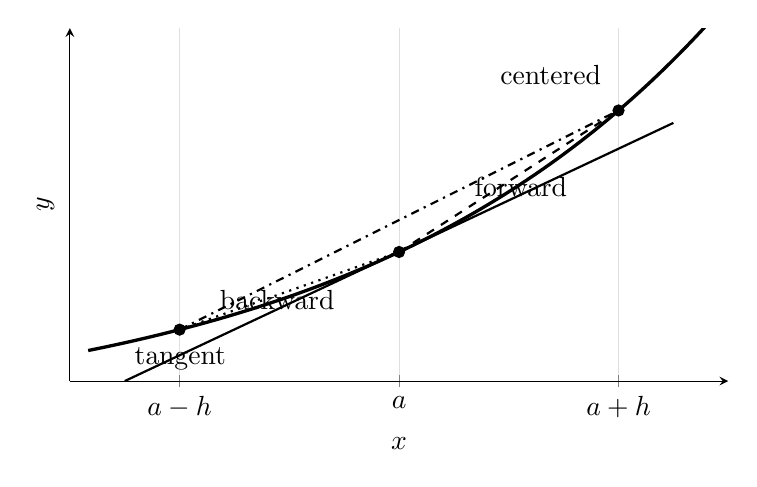
\begin{tikzpicture}
\begin{axis}[
    width=0.82\textwidth,
    height=0.50\textwidth,
    xmin=-0.9, xmax=0.9,
    ymin=0.25, ymax=2.3,
    axis lines=left,
    xlabel={\(x\)},
    ylabel={\(y\)},
    xtick={-0.6,0,0.6},
    xticklabels={\(a-h\),\(a\),\(a+h\)},
    ytick=\empty,
    grid=both,
    grid style={line width=.1pt, draw=gray!25},
]
\addplot[very thick, domain=-0.85:0.85, samples=150] {exp(x)};
\addplot[thick, dashed] coordinates {(0,1) (0.6,1.82212)};
\addplot[thick, dotted] coordinates {(-0.6,0.54881) (0,1)};
\addplot[thick, dashdotted] coordinates {(-0.6,0.54881) (0.6,1.82212)};
\addplot[thick, domain=-0.75:0.75, samples=2] {1+x};
\addplot[only marks, mark=*] coordinates {(-0.6,0.54881) (0,1) (0.6,1.82212)};

\node[anchor=west] at (axis cs:0.18,1.38) {forward};
\node[anchor=east] at (axis cs:-0.15,0.72) {backward};
\node[anchor=west] at (axis cs:0.25,2.03) {centered};
\node[anchor=west] at (axis cs:-0.75,0.38) {tangent};
\end{axis}
\end{tikzpicture}
\caption{Forward, backward, and centered differences approximate the tangent slope using nearby secant slopes.}
\label{fig:finite-difference-secants}
\end{figure}

\paragraph{Example: differentiating from values.}
Estimate

\[
\frac{d}{dx}e^x\Big|_{x=0}
\]

using \(h=0.1\).

The true derivative is

\[
\left(e^x\right)'=e^x,
\]

so

\[
f'(0)=1.
\]

Now compare the numerical approximations.

The forward difference is

\[
D_{0.1}^+f(0)
=
\frac{e^{0.1}-e^0}{0.1}
=
\frac{1.105171-1}{0.1}
=
1.051709.
\]

The backward difference is

\[
D_{0.1}^-f(0)
=
\frac{e^0-e^{-0.1}}{0.1}
=
\frac{1-0.904837}{0.1}
=
0.951626.
\]

The centered difference is

\[
D_{0.1}^0f(0)
=
\frac{e^{0.1}-e^{-0.1}}{0.2}
=
\frac{1.105171-0.904837}{0.2}
=
1.001668.
\]

\begin{center}
\begin{tabular}{c|c|c}
\textbf{method} & \textbf{approximation} & \textbf{absolute error} \\ \hline
forward difference & \(1.051709\) & \(0.051709\) \\
backward difference & \(0.951626\) & \(0.048374\) \\
centered difference & \(1.001668\) & \(0.001668\)
\end{tabular}
\end{center}

The centered difference is much better here because the errors from the left and right
partly cancel.

\subsection{Truncation error}
\label{subsec:truncation-error}

A finite-difference formula replaces a limit by a finite step.  The error from doing that
is called \emph{truncation error}.

The word means: we stopped a limiting process early.

To see the size of the error, expand \(f(a+h)\) near \(a\).  Taylor's formula gives

\[
f(a+h)
=
f(a)+f'(a)h+\frac12f''(a)h^2+\frac16f'''(a)h^3+\cdots.
\]

For the forward difference,

\[
\frac{f(a+h)-f(a)}{h}
=
f'(a)+\frac12f''(a)h+\frac16f'''(a)h^2+\cdots.
\]

So

\[
\boxed{
D_h^+f(a)=f'(a)+\frac12f''(a)h+\text{terms involving }h^2,h^3,\ldots
}
\]

The leading error is usually proportional to \(h\).

For the backward difference,

\[
f(a-h)
=
f(a)-f'(a)h+\frac12f''(a)h^2-\frac16f'''(a)h^3+\cdots.
\]

Therefore

\[
\frac{f(a)-f(a-h)}{h}
=
f'(a)-\frac12f''(a)h+\frac16f'''(a)h^2-\cdots.
\]

So

\[
\boxed{
D_h^-f(a)=f'(a)-\frac12f''(a)h+\text{terms involving }h^2,h^3,\ldots
}
\]

The forward and backward errors have opposite first-order terms.

Now subtract the Taylor expansions:

\[
f(a+h)-f(a-h)
=
2f'(a)h+\frac13f'''(a)h^3+\cdots.
\]

Divide by \(2h\):

\[
\frac{f(a+h)-f(a-h)}{2h}
=
f'(a)+\frac16f'''(a)h^2+\cdots.
\]

Thus

\[
\boxed{
D_h^0f(a)=f'(a)+\frac16f'''(a)h^2+\text{terms involving }h^4,h^6,\ldots
}
\]

The leading error is usually proportional to \(h^2\).

\begin{quote}
\textbf{Truncation error pattern.}

For smooth functions,

\[
D_h^+f(a)-f'(a)
\quad\text{and}\quad
D_h^-f(a)-f'(a)
\]

are usually of size roughly proportional to \(h\), while

\[
D_h^0f(a)-f'(a)
\]

is usually of size roughly proportional to \(h^2\).
\end{quote}

This explains why centered differences are often much better than one-sided differences
when the same step size is used.

\paragraph{Example: why the centered error is small.}
For \(f(x)=e^x\), all derivatives equal \(e^x\).  At \(a=0\),

\[
f'(0)=f''(0)=f'''(0)=1.
\]

The forward difference has leading error approximately

\[
\frac12h.
\]

With \(h=0.1\), this predicts error near

\[
0.05,
\]

which matches the observed forward error

\[
0.051709.
\]

The centered difference has leading error approximately

\[
\frac16h^2.
\]

With \(h=0.1\), this predicts error near

\[
\frac{0.01}{6}=0.001667,
\]

which matches the observed centered error

\[
0.001668.
\]

The Taylor expansion is not only a formal calculation.  It tells us how the error behaves.

\subsection{Roundoff error}
\label{subsec:roundoff-error}

Truncation error suggests a simple strategy:

\[
\text{make \(h\) smaller.}
\]

But computation has another error source.

A computer does not usually store real numbers exactly.  It stores rounded
approximations.  When two nearly equal rounded numbers are subtracted, the small
difference may lose important digits.

That is exactly what finite differences do.

\[
f(a+h)-f(a)
\]

subtracts two nearby values.  When \(h\) is very small, these values are very close.

Suppose the computed values of \(f(a+h)\) and \(f(a)\) each have possible absolute
error at most \(\eta\).  Then the numerator

\[
f(a+h)-f(a)
\]

may have error as large as approximately

\[
2\eta.
\]

After dividing by \(h\), the derivative approximation may have roundoff error as large
as

\[
\frac{2\eta}{h}.
\]

So roundoff error grows as \(h\) shrinks.

\[
\boxed{
\text{Small \(h\) reduces truncation error but can increase roundoff error.}
}
\]

This is the central tension in numerical differentiation.

\paragraph{A typical floating-point experiment.}
Compute

\[
\frac{e^h-1}{h}
\]

as an approximation to \(f'(0)\) for \(f(x)=e^x\).  The true value is \(1\).

A typical double-precision computation may look like this:

\[
\begin{array}{c|c|c}
h & \dfrac{e^h-1}{h} & \text{absolute error} \\ \hline
10^{-1} & 1.0517091808 & 5.17\cdot10^{-2} \\
10^{-4} & 1.0000500017 & 5.00\cdot10^{-5} \\
10^{-8} & 0.9999999939 & 6.08\cdot10^{-9} \\
10^{-10} & 1.0000000827 & 8.27\cdot10^{-8} \\
10^{-12} & 1.0000889006 & 8.89\cdot10^{-5}
\end{array}
\]

At first the error decreases.  Then it increases.

The mathematical limit is still true:

\[
\lim_{h\to0}\frac{e^h-1}{h}=1.
\]

But the computer is not taking a mathematical limit.  It is doing arithmetic with rounded
numbers.

\subsection{Why smaller \texorpdfstring{\(h\)}{h} is not always better}
\label{subsec:why-smaller-h-not-always-better}

There are two competing errors.

For a forward difference,

\[
\text{truncation error}\approx C_1h,
\]

while

\[
\text{roundoff error}\approx \frac{C_2\eta}{h}.
\]

So a rough total error model is

\[
\boxed{
\text{total error}\approx C_1h+\frac{C_2\eta}{h}.
}
\]

The first term decreases when \(h\) decreases.  The second term increases when \(h\)
decreases.

There is usually a best middle range.

For a centered difference,

\[
\text{truncation error}\approx C_1h^2,
\]

while roundoff still behaves like

\[
\frac{C_2\eta}{h}.
\]

So centered differences often allow a smaller error before roundoff takes over, but they
do not escape the problem entirely.

\begin{quote}
\textbf{Practical lesson.}

For numerical derivatives, do not blindly make \(h\) extremely small.

Use a moderately small \(h\), compare several step sizes, and prefer centered differences
when the data allow them.
\end{quote}

\subsection{Data, endpoints, and one-sided differences}
\label{subsec:data-endpoints-one-sided-differences}

Experimental data often come in a table.

\[
\begin{array}{c|ccccc}
t & 0 & 1 & 2 & 3 & 4 \\ \hline
s(t) & 0.0 & 1.8 & 7.9 & 18.2 & 32.1
\end{array}
\]

If \(s(t)\) is position, then finite differences estimate velocity.

At \(t=2\), the centered difference with \(h=1\) is

\[
\frac{s(3)-s(1)}{2}
=
\frac{18.2-1.8}{2}
=
8.2.
\]

So the estimated velocity at \(t=2\) is

\[
8.2
\]

position units per time unit.

At the left endpoint \(t=0\), a centered difference using \(t=-1\) is not available.  We
may use a forward difference:

\[
\frac{s(1)-s(0)}{1}
=
1.8.
\]

At the right endpoint \(t=4\), we may use a backward difference:

\[
\frac{s(4)-s(3)}{1}
=
13.9.
\]

\begin{center}
\begin{tabular}{c|c|c}
\textbf{point} & \textbf{available estimate} & \textbf{reason} \\ \hline
left endpoint & forward difference & no data to the left \\
interior point & centered difference & data on both sides \\
right endpoint & backward difference & no data to the right
\end{tabular}
\end{center}

This is common in applications.  The best formula is not only a matter of accuracy.
It also depends on which measurements are available.

\subsection{Warning example: a difference quotient may hide a corner}
\label{subsec:difference-quotient-hide-corner}

Numerical differentiation can produce a number even when the derivative does not
exist.

Let

\[
f(x)=|x|.
\]

At \(x=0\), the graph has a corner.  The derivative does not exist.

The forward difference is

\[
D_h^+f(0)=\frac{|h|-|0|}{h}=1
\]

for \(h>0\).

The backward difference is

\[
D_h^-f(0)=\frac{|0|-|-h|}{h}=-1.
\]

The centered difference is

\[
D_h^0f(0)=\frac{|h|-|-h|}{2h}=0.
\]

So the three numerical formulas give

\[
1,\qquad -1,\qquad 0.
\]

None of these means that \(f'(0)\) exists.

\begin{figure}[h]
\centering
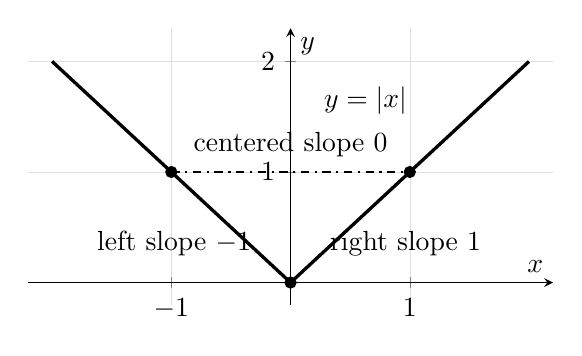
\begin{tikzpicture}
\begin{axis}[
    width=0.68\textwidth,
    height=0.42\textwidth,
    xmin=-2.2, xmax=2.2,
    ymin=-0.2, ymax=2.3,
    axis lines=middle,
    xlabel={\(x\)},
    ylabel={\(y\)},
    xtick={-1,0,1},
    ytick={0,1,2},
    grid=both,
    grid style={line width=.1pt, draw=gray!25},
]
\addplot[very thick, domain=-2:0, samples=2] {-x};
\addplot[very thick, domain=0:2, samples=2] {x};
\addplot[thick, dashed] coordinates {(0,0) (1,1)};
\addplot[thick, dotted] coordinates {(-1,1) (0,0)};
\addplot[thick, dashdotted] coordinates {(-1,1) (1,1)};
\addplot[only marks, mark=*] coordinates {(-1,1) (0,0) (1,1)};
\node[anchor=west] at (axis cs:0.2,1.65) {\(y=|x|\)};
\node[anchor=west] at (axis cs:0.25,0.35) {right slope \(1\)};
\node[anchor=east] at (axis cs:-0.25,0.35) {left slope \(-1\)};
\node[anchor=south] at (axis cs:0,1.05) {centered slope \(0\)};
\end{axis}
\end{tikzpicture}
\caption{For \(f(x)=|x|\), the centered difference at \(0\) equals \(0\), but the derivative at \(0\) does not exist.}
\label{fig:centered-difference-absolute-value}
\end{figure}

\begin{quote}
\textbf{Warning.}
A finite-difference formula can return a number even when the derivative does not
exist.

Numerical evidence must be interpreted with the graph, the data, and the hypotheses
in mind.
\end{quote}

This warning is especially important with noisy data.  If the measurements contain
small errors, dividing by a small \(h\) can turn small measurement errors into large
derivative errors.

Differentiation magnifies noise.  Integration averages noise.

That is one reason numerical differentiation is usually more delicate than numerical
integration.

\subsection{Where this points}
\label{subsec:numerical-differentiation-hook-newton-revisited}

Numerical integration and numerical differentiation both replace a limit by a finite
calculation.  Each method has an error story.

For integration, smaller subintervals usually improve the approximation, and the error
bounds can be very strong for smooth functions.

For differentiation, smaller steps reduce truncation error but may increase roundoff
error.  The best computation is a compromise.

The next natural place where approximation, derivatives, and error meet is Newton's
method.  We already used Newton's method to find roots.  Now we can ask sharper
computational questions:

\[
\text{When should the iteration stop?}
\]

\[
\text{How close is the current guess to the root?}
\]

\[
\text{What happens when the derivative is small or the root is repeated?}
\]

Those questions bring Newton's method back, this time as a numerical algorithm rather
than only a tangent-line idea.
\section{Newton's method revisited}
\label{sec:newtons-method-revisited}

Numerical differentiation taught us a useful warning: a formula can be mathematically
correct and still be delicate in computation.  Newton's method has the same personality.

Earlier, Newton's method came from tangent lines.  To solve

\[
f(x)=0,
\]

we replaced the curve by its tangent line at a current guess \(x_n\), then used the
\(x\)-intercept of that tangent line as the next guess:

\[
\boxed{
x_{n+1}=x_n-\frac{f(x_n)}{f'(x_n)}.
}
\]

That formula is simple.  The computational questions are not.

\[
\text{When should we stop?}
\]

\[
\text{How close is the current guess to the root?}
\]

\[
\text{What changes when the root is multiple?}
\]

\[
\text{What can go wrong if we iterate from a bad starting point?}
\]

These are not side questions.  They are the questions that turn Newton's method from a
geometric idea into a numerical algorithm.

\subsection{Stopping criteria}
\label{subsec:newton-stopping-criteria}

A computer almost never lands on the exact root.  It produces a sequence

\[
x_0,\ x_1,\ x_2,\ \ldots
\]

and we must decide when the sequence is good enough.

There are two numbers we can easily monitor.

First, we can monitor the residual:

\[
|f(x_n)|.
\]

This tells us how close the function value is to \(0\).

Second, we can monitor the step size:

\[
|x_n-x_{n-1}|.
\]

This tells us how much the iterates are still moving.

Both are useful.  Neither is perfect by itself.

\paragraph{Example: square root of \(2\).}
To compute \(\sqrt2\), solve

\[
f(x)=x^2-2=0.
\]

Newton's method gives

\[
x_{n+1}
=
x_n-\frac{x_n^2-2}{2x_n}
=
\frac12\left(x_n+\frac2{x_n}\right).
\]

Start with

\[
x_0=1.5.
\]

The iterates are:

\begin{center}
\begin{tabular}{c|c|c|c}
\(n\) & \(x_n\) & \(|f(x_n)|\) & \(|x_n-x_{n-1}|\) \\ \hline
\(0\) & \(1.500000000\) & \(2.500000\cdot10^{-1}\) & -- \\
\(1\) & \(1.416666667\) & \(6.944444\cdot10^{-3}\) & \(8.333333\cdot10^{-2}\) \\
\(2\) & \(1.414215686\) & \(6.007305\cdot10^{-6}\) & \(2.450980\cdot10^{-3}\) \\
\(3\) & \(1.414213562\) & \(4.510614\cdot10^{-12}\) & \(2.123900\cdot10^{-6}\) \\
\(4\) & \(1.414213562\) & \(4.440892\cdot10^{-16}\) & \(1.594946\cdot10^{-12}\)
\end{tabular}
\end{center}

By \(n=3\), both the residual and the step size are tiny.  The sequence has stabilized
for any ordinary decimal purpose.

\begin{quote}
\textbf{A practical stopping rule.}
Choose tolerances \(\varepsilon_{\text{res}}>0\) and \(\varepsilon_{\text{step}}>0\).  Stop when

\[
|f(x_n)|<\varepsilon_{\text{res}}
\]

and

\[
|x_n-x_{n-1}|<\varepsilon_{\text{step}}.
\]

Also choose a maximum number of iterations, so the method cannot run forever.
\end{quote}

A typical algorithm therefore asks for three pieces of numerical judgment:

\[
\text{residual tolerance},\qquad
\text{step tolerance},\qquad
\text{maximum number of iterations}.
\]

The maximum iteration count is not mathematical decoration.  It protects us from
cycles, divergence, and programming mistakes.

\paragraph{Why residual alone can mislead.}
A small residual does not always mean a small error in \(x\).  The reason is slope.

If the graph is very flat near the axis, then the function value can be small even when
the input is not very close to the root.

For example, consider

\[
f(x)=10^{-8}(x-10^6).
\]

The root is

\[
r=10^6.
\]

At \(x=0\),

\[
f(0)=-10^{-2}.
\]

If a careless stopping rule accepts every residual less than \(0.02\), then \(x=0\) would
be accepted even though it is one million units away from the root.

The residual must be interpreted together with the scale of the function and the slope
near the root.

\[
\boxed{
\text{Small \(f(x_n)\) is strongest evidence when \(f'\) is not small near the root.}
}
\]

\paragraph{Why step size alone can mislead.}
A small step size can also be misleading.  An iteration may stop moving because of
roundoff error, because the derivative is badly scaled, or because the method is trapped
near a point that is not a root.

So a step-size test should usually be paired with a residual test.  We want the iterates to
stop moving \emph{and} the function value to be close to zero.

\subsection{Error estimates}
\label{subsec:newton-error-estimates}

A residual is easy to compute.  The actual error

\[
|x_n-r|
\]

is usually not easy to compute, because the root \(r\) is the thing we are trying to find.

Still, we can sometimes bound the error.

Suppose \(r\) is a root, so

\[
f(r)=0.
\]

If \(x_n\) and \(r\) lie in an interval where

\[
|f'(x)|\ge m>0,
\]

then the Mean Value Theorem gives

\[
|f(x_n)-f(r)|=|f'(c)|\,|x_n-r|
\]

for some \(c\) between \(x_n\) and \(r\).  Since \(f(r)=0\),

\[
|f(x_n)|=|f'(c)|\,|x_n-r|.
\]

Because \(|f'(c)|\ge m\), we get

\[
\boxed{
|x_n-r|\le \frac{|f(x_n)|}{m}.
}
\]

This is an \emph{a posteriori} error estimate: it uses information from the approximation
we have already computed.

\paragraph{Example: residual gives an error bound.}
Suppose we use Newton's method on

\[
f(x)=x^2-2
\]

and obtain

\[
x_3=1.4142135623746899.
\]

We know the positive root lies between \(1\) and \(2\).  On this interval,

\[
f'(x)=2x,
\]

so

\[
|f'(x)|\ge 2.
\]

The residual is approximately

\[
|f(x_3)|\approx 4.51\cdot10^{-12}.
\]

Therefore

\[
|x_3-\sqrt2|
\le
\frac{4.51\cdot10^{-12}}{2}
=
2.26\cdot10^{-12}.
\]

So the approximation is guaranteed to be within about

\[
2.26\cdot10^{-12}
\]

of the true root.

This bound is not the same thing as the actual error.  It is a guarantee based on a lower
bound for the derivative.

\subsection{The Newton step as an error estimate}
\label{subsec:newton-step-error-estimate}

The Newton step is

\[
s_n=x_{n+1}-x_n=-\frac{f(x_n)}{f'(x_n)}.
\]

Near a simple root, the tangent line predicts that the root is approximately

\[
x_n+s_n.
\]

So

\[
|s_n|
\]

is often a rough estimate of the current error \(|x_n-r|\).

This is why the step size is useful as a stopping test.  If the next tangent correction is
tiny, then the current approximation is probably close to a root, provided the residual is
also tiny and the derivative is not causing trouble.

But there is something even better near a simple root.

Earlier, Taylor's formula gave the Newton error relation

\[
x_{n+1}-r
=
\frac{f''(c_n)}{2f'(x_n)}(r-x_n)^2
\]

for some point \(c_n\) between \(x_n\) and \(r\).  So near a simple root,

\[
\boxed{
|x_{n+1}-r|\approx C|x_n-r|^2.
}
\]

This is \emph{quadratic convergence}.

If the current error is about \(10^{-3}\), the next error may be about \(10^{-6}\).  If the
current error is about \(10^{-6}\), the next error may be about \(10^{-12}\).

That is why Newton's method can suddenly gain many digits.

\begin{quote}
\textbf{Practical lesson.}
When Newton's method is converging well to a simple root, the number of correct
digits often roughly doubles from one step to the next.

When it is not converging well, no stopping rule should pretend that it is.
\end{quote}

\subsection{Multiple roots}
\label{subsec:newton-multiple-roots-revisited}

Newton's method is fastest near a \emph{simple} root.  A simple root is a root \(r\) for
which

\[
f(r)=0
\qquad\text{and}\qquad
f'(r)\neq0.
\]

If

\[
f'(r)=0,
\]

then the graph touches the axis more flatly.  Newton's method may still converge, but
the convergence often becomes much slower.

\paragraph{Example: a double root.}
Let

\[
f(x)=(x-1)^2.
\]

The root is

\[
r=1,
\]

and it is a double root.  Since

\[
f'(x)=2(x-1),
\]

we have

\[
f'(1)=0.
\]

Newton's method gives, for \(x_n\neq1\),

\[
x_{n+1}
=
x_n-\frac{(x_n-1)^2}{2(x_n-1)}.
\]

Cancel one factor:

\[
x_{n+1}
=
x_n-\frac{x_n-1}{2}.
\]

So

\[
\boxed{
x_{n+1}=\frac{x_n+1}{2}.
}
\]

Starting from \(x_0=2\), the iterates are:

\begin{center}
\begin{tabular}{c|c|c}
\(n\) & \(x_n\) & \(|x_n-1|\) \\ \hline
\(0\) & \(2.000000\) & \(1.000000\) \\
\(1\) & \(1.500000\) & \(0.500000\) \\
\(2\) & \(1.250000\) & \(0.250000\) \\
\(3\) & \(1.125000\) & \(0.125000\) \\
\(4\) & \(1.062500\) & \(0.062500\)
\end{tabular}
\end{center}

The error is cut in half each time.  That is convergence, but it is not quadratic
convergence.  It is only linear convergence.

\begin{figure}[h]
\centering
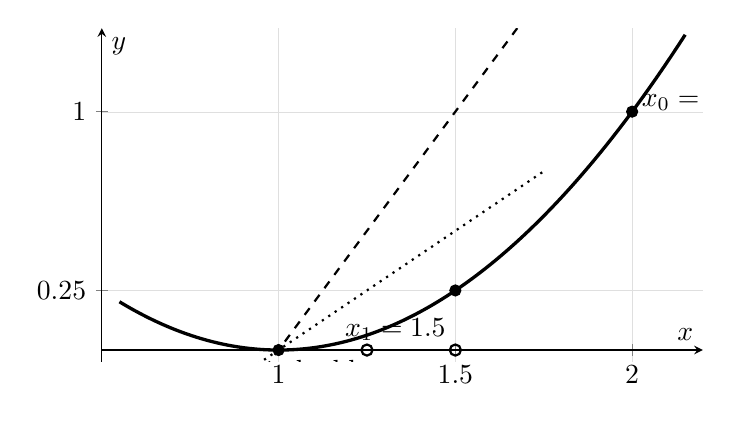
\begin{tikzpicture}
\begin{axis}[
    width=0.76\textwidth,
    height=0.48\textwidth,
    xmin=0.5, xmax=2.2,
    ymin=-0.05, ymax=1.35,
    axis lines=middle,
    xlabel={\(x\)},
    ylabel={\(y\)},
    xtick={1,1.5,2},
    ytick={0,0.25,1},
    grid=both,
    grid style={line width=.1pt, draw=gray!25},
]
\addplot[very thick, domain=0.55:2.15, samples=150] {(x-1)^2};
% tangent at x=2: y=2(x-1)
\addplot[thick, dashed, domain=0.85:2.1, samples=2] {2*(x-1)};
% tangent at x=1.5: y=(x-1)
\addplot[thick, dotted, domain=0.85:1.75, samples=2] {x-1};
\addplot[only marks, mark=*] coordinates {(2,1) (1.5,0.25) (1,0)};
\addplot[only marks, mark=o, thick] coordinates {(1.5,0) (1.25,0)};
\node[anchor=west] at (axis cs:2,1.05) {\(x_0=2\)};
\node[anchor=south east] at (axis cs:1.5,0) {\(x_1=1.5\)};
\node[anchor=north west] at (axis cs:1,0) {double root};
\end{axis}
\end{tikzpicture}
\caption{At a double root, the graph is tangent to the \(x\)-axis.  Newton's method still moves toward the root, but much more slowly.}
\label{fig:newton-double-root}
\end{figure}

The same pattern appears for higher multiplicity.  If

\[
f(x)=(x-r)^m,
\]

then

\[
f'(x)=m(x-r)^{m-1}.
\]

Newton's method gives

\[
x_{n+1}
=
x_n-\frac{(x_n-r)^m}{m(x_n-r)^{m-1}}
=
x_n-\frac{x_n-r}{m}.
\]

Therefore

\[
x_{n+1}-r
=
\left(1-\frac1m\right)(x_n-r).
\]

So the error is multiplied by

\[
1-\frac1m
\]

each step.

For a double root, this factor is \(1/2\).  For a triple root, it is \(2/3\).  The larger the
multiplicity, the slower the basic Newton iteration becomes.

\begin{quote}
\textbf{Multiple-root warning.}
If Newton's method converges only linearly, one possible reason is that the root is
multiple.

Repeatedly small residuals with slow-moving iterates may indicate a flat crossing or
a flat touch near the axis.
\end{quote}

If the multiplicity \(m\) is known, a modified Newton step can help:

\[
\boxed{
x_{n+1}=x_n-m\frac{f(x_n)}{f'(x_n)}.
}
\]

For

\[
f(x)=(x-r)^m,
\]

this modified method reaches the root in one step.  For more general functions with a
root of multiplicity \(m\), it can restore much faster convergence near the root.

But the multiplicity is not always known.  That is why observing the behavior of the
iteration matters.

\subsection{A first glimpse of chaotic iteration}
\label{subsec:first-glimpse-chaotic-iteration}

Newton's method is an iteration:

\[
x_{n+1}=N(x_n),
\]

where

\[
N(x)=x-\frac{f(x)}{f'(x)}.
\]

So Newton's method is not only a root-finding formula.  It is also a dynamical system:
a rule that sends each point to a next point.

When the starting point is close to a simple root, the dynamics are friendly.  The root
attracts nearby iterates.

Far from a root, the dynamics can be complicated.

\paragraph{Example: asking for a real root that does not exist.}
Let

\[
f(x)=x^2+1.
\]

This function has no real root.  Still, Newton's formula produces an iteration.

Since

\[
f'(x)=2x,
\]

we get

\[
x_{n+1}
=
x_n-\frac{x_n^2+1}{2x_n}.
\]

Simplify:

\[
\boxed{
x_{n+1}
=
\frac12\left(x_n-\frac1{x_n}\right).
}
\]

This formula is defined whenever \(x_n\neq0\).

Start with

\[
x_0=1.
\]

Then

\[
x_1=\frac12(1-1)=0.
\]

The next step is impossible because the formula would require division by \(0\).

Start instead with

\[
x_0=1.01.
\]

Then

\[
x_1
=
\frac12\left(1.01-\frac1{1.01}\right)
\approx 0.0099505.
\]

Now the next step contains \(1/x_1\), which is huge:

\[
x_2
\approx
\frac12(0.0099505-100.4975)
\approx -50.2438.
\]

A tiny change from \(1\) to \(1.01\) has produced a very different next story.

\begin{figure}[h]
\centering
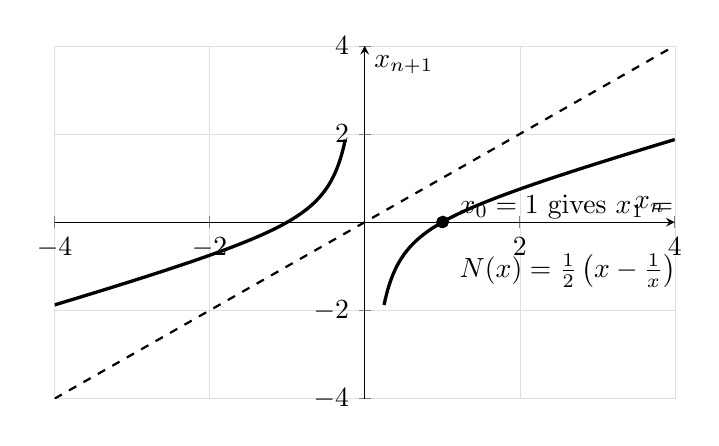
\begin{tikzpicture}
\begin{axis}[
    width=0.78\textwidth,
    height=0.50\textwidth,
    xmin=-4, xmax=4,
    ymin=-4, ymax=4,
    axis lines=middle,
    xlabel={\(x_n\)},
    ylabel={\(x_{n+1}\)},
    xtick={-4,-2,0,2,4},
    ytick={-4,-2,0,2,4},
    grid=both,
    grid style={line width=.1pt, draw=gray!25},
]
\addplot[very thick, domain=-4:-0.25, samples=200] {0.5*(x-1/x)};
\addplot[very thick, domain=0.25:4, samples=200] {0.5*(x-1/x)};
\addplot[thick, dashed, domain=-4:4, samples=2] {x};
\addplot[only marks, mark=*] coordinates {(1,0) (1.01,0.0099505)};
\node[anchor=west] at (axis cs:1.1,0.35) {\(x_0=1\) gives \(x_1=0\)};
\node[anchor=west] at (axis cs:1.1,-1.1) {\(N(x)=\frac12\left(x-\frac1x\right)\)};
\end{axis}
\end{tikzpicture}
\caption{Newton's method for \(x^2+1=0\) over the real numbers produces the iteration \(N(x)=\frac12(x-1/x)\).  There is no real root to attract the iterates.}
\label{fig:newton-map-x2-plus-1}
\end{figure}

This example is not here because we need to solve \(x^2+1=0\) over the real numbers.
We already know there is no real solution.

It is here because it shows something deeper: an iteration can have a simple rule and
complicated behavior.

\begin{quote}
\textbf{Computational warning.}
Newton's method can be extremely fast near a good root.  Far from a good root, it can
move to a different root, enter a cycle, become undefined, or behave unpredictably.

Always monitor the iterates.
\end{quote}

This warning does not make Newton's method less valuable.  It makes it more honest.
In serious computation, a fast method and a safety check belong together.

\subsection{A safe Newton workflow}
\label{subsec:safe-newton-workflow}

When using Newton's method as a numerical algorithm, follow a disciplined workflow.

\begin{enumerate}
\item Choose a function \(f\) whose root solves the original problem.

\item Choose a starting value \(x_0\) from a graph, table, physical estimate, or bracket.

\item Compute

\[
x_{n+1}=x_n-\frac{f(x_n)}{f'(x_n)}
\]

only when \(f'(x_n)\neq0\).

\item At each step, record \(x_n\), \(f(x_n)\), and \(x_n-x_{n-1}\).

\item Stop only when the residual and step size are both small enough.

\item If the method leaves the physical domain, cycles, or fails to reduce the residual,
restart with a better initial guess or use a safer method such as bisection.
\end{enumerate}

Newton's method is a perfect example of this chapter's theme.  Calculus gives the idea:
follow the tangent line.  Computation adds the discipline: check whether the idea is
working.

The same discipline belongs to numerical integration.  We have formulas, but formulas
become understanding only when we test them.

\section{Computing experiments}
\label{sec:computing-experiments}

Numerical methods become real when we use them.

The purpose of these experiments is not only to produce decimals.  A calculator can
produce decimals.  The purpose is to learn how numerical answers behave when the
step size changes, when the function becomes less smooth, and when an algorithm is
implemented by an actual person or machine.

Each experiment follows the same pattern:

\[
\text{compute},\qquad
\text{compare},\qquad
\text{explain}.
\]

\subsection{Experiment 1: approximate \texorpdfstring{\(\pi\)}{pi} by integration}
\label{subsec:experiment-approximate-pi}

The number \(\pi\) can be computed from an integral.

Since

\[
\frac{d}{dx}\arctan x=\frac{1}{1+x^2},
\]

we have

\[
\int_0^1 \frac{1}{1+x^2}\,dx
=
\arctan(1)-\arctan(0)
=
\frac{\pi}{4}.
\]

Therefore

\[
\boxed{
\pi=4\int_0^1 \frac{1}{1+x^2}\,dx.
}
\]

So we can approximate \(\pi\) by approximating the integral

\[
\int_0^1 \frac{4}{1+x^2}\,dx.
\]

Let

\[
f(x)=\frac{4}{1+x^2}.
\]

Use the midpoint rule, trapezoidal rule, and Simpson's Rule on \([0,1]\).

\begin{center}
\begin{tabular}{c|c|c|c}
\(n\) & \(M_n\) & \(T_n\) & \(S_n\) \\ \hline
\(4\) & \(3.146801\) & \(3.131176\) & \(3.141569\) \\
\(8\) & \(3.142895\) & \(3.138988\) & \(3.141593\) \\
\(16\) & \(3.141918\) & \(3.140942\) & \(3.141593\) \\
\(32\) & \(3.141674\) & \(3.141430\) & \(3.141593\)
\end{tabular}
\end{center}

The true value begins

\[
\pi=3.1415926535\ldots.
\]

Simpson's Rule performs very well here because the integrand is smooth on the whole
interval.

\paragraph{Project tasks.}
Complete the following.

\begin{enumerate}
\item Reproduce the table above using a calculator, spreadsheet, or program.

\item Add a column for the absolute error

\[
|\pi-\text{approximation}|.
\]

\item When \(n\) doubles, how does the error change for each rule?

\item Which rule gives the best answer for the same \(n\)?

\item Which rule gives the best answer for the same number of function evaluations?

\item Use the Simpson error bound to explain why the Simpson values stabilize so
quickly.

\item Repeat the experiment using the quarter-circle formula

\[
\pi=4\int_0^1 \sqrt{1-x^2}\,dx.
\]

Which formula is numerically friendlier?  Why might the endpoint \(x=1\) cause
trouble for error bounds?
\end{enumerate}

The last question is important.  Two different integrals can equal the same number, but
they may not be equally good for computation.

\subsection{Experiment 2: estimate a probability from a density}
\label{subsec:experiment-probability-density}

A probability density is a function whose accumulated area gives probability.

The standard normal density is

\[
\phi(x)=\frac{1}{\sqrt{2\pi}}e^{-x^2/2}.
\]

It is centered at \(0\), symmetric, and bell-shaped.

The probability that a standard normal quantity lies between \(-1\) and \(1\) is

\[
P(-1\le Z\le1)
=
\int_{-1}^{1}
\frac{1}{\sqrt{2\pi}}e^{-x^2/2}\,dx.
\]

This integral has no elementary antiderivative.  Numerical integration is the natural
tool.

Using Simpson's Rule gives:

\begin{center}
\begin{tabular}{c|c}
\(n\) & Simpson approximation to \(P(-1\le Z\le1)\) \\ \hline
\(4\) & \(0.683058\) \\
\(8\) & \(0.682711\) \\
\(16\) & \(0.682691\) \\
\(32\) & \(0.682690\)
\end{tabular}
\end{center}

A more refined computation gives approximately

\[
P(-1\le Z\le1)\approx0.682689.
\]

So about \(68.27\%\) of the probability lies within one standard deviation of the mean.

\begin{figure}[h]
\centering
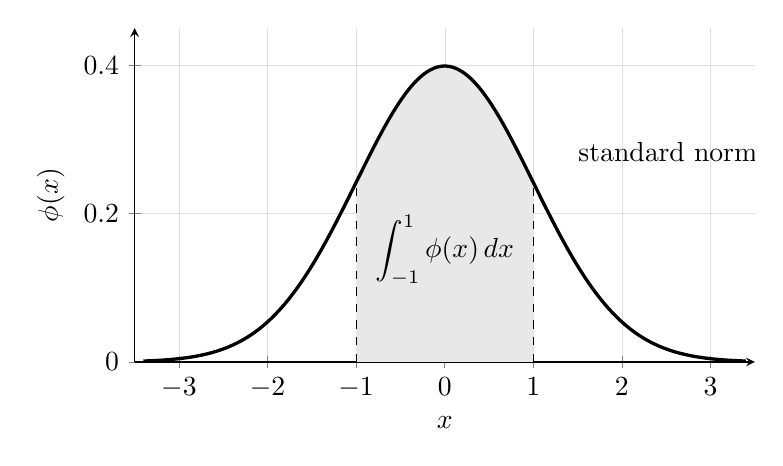
\begin{tikzpicture}
\begin{axis}[
    width=0.78\textwidth,
    height=0.48\textwidth,
    xmin=-3.5, xmax=3.5,
    ymin=0, ymax=0.45,
    axis lines=left,
    xlabel={\(x\)},
    ylabel={\(\phi(x)\)},
    xtick={-3,-2,-1,0,1,2,3},
    ytick={0,0.2,0.4},
    grid=both,
    grid style={line width=.1pt, draw=gray!25},
]
\addplot[domain=-1:1, samples=150, fill=gray!18, draw=none]
  {1/sqrt(2*pi)*exp(-x^2/2)} \closedcycle;
\addplot[very thick, domain=-3.4:3.4, samples=250]
  {1/sqrt(2*pi)*exp(-x^2/2)};
\draw[dashed] (axis cs:-1,0) -- (axis cs:-1,{1/sqrt(2*pi)*exp(-0.5)});
\draw[dashed] (axis cs:1,0) -- (axis cs:1,{1/sqrt(2*pi)*exp(-0.5)});
\node[anchor=south] at (axis cs:0,0.09)
  {\(\displaystyle \int_{-1}^{1}\phi(x)\,dx\)};
\node[anchor=west] at (axis cs:1.4,0.28) {standard normal density};
\end{axis}
\end{tikzpicture}
\caption{For a probability density, area under the curve is probability.}
\label{fig:normal-density-probability}
\end{figure}

\paragraph{Project tasks.}
Complete the following.

\begin{enumerate}
\item Use the midpoint, trapezoidal, and Simpson rules to approximate

\[
\int_{-1}^{1}\phi(x)\,dx.
\]

Use \(n=4,8,16,32\).

\item Compare your answers with

\[
0.682689.
\]

\item Use symmetry to explain why

\[
\int_{-1}^{1}\phi(x)\,dx
=
2\int_0^1\phi(x)\,dx.
\]

\item Estimate

\[
\int_{-2}^{2}\phi(x)\,dx.
\]

How much larger is this probability?

\item Estimate

\[
\int_{-4}^{4}\phi(x)\,dx.
\]

Why is this close to \(1\), even though the true total probability is the improper
integral

\[
\int_{-\infty}^{\infty}\phi(x)\,dx?
\]
\end{enumerate}

This experiment connects three ideas: numerical integration, improper integrals, and
probability.

\subsection{Experiment 3: compare rules on smooth and rough functions}
\label{subsec:experiment-smooth-rough}

Error bounds have hypotheses.  Simpson's Rule needs a bounded fourth derivative for
its standard error bound.  The midpoint and trapezoidal bounds need a bounded second
derivative.

Smooth functions reward high-order methods.  Less smooth functions may not.

Compare these two integrals:

\[
I_1=\int_0^1 e^{-x^2}\,dx
\]

and

\[
I_2=\int_0^1 \sqrt{x}\,dx.
\]

The first integrand is smooth.  The second is continuous, but its derivatives become
large near \(x=0\).  In fact,

\[
\frac{d^2}{dx^2}\sqrt{x}
=
-\frac{1}{4x^{3/2}}
\]

for \(x>0\), which is unbounded near \(0\).

The exact value of \(I_2\) is

\[
I_2=\frac23.
\]

A refined value of \(I_1\) is

\[
I_1\approx0.7468241328.
\]

Using Simpson's Rule gives the following comparison.

\begin{center}
\begin{tabular}{c|c|c}
\(n\) & Simpson for \(\int_0^1 e^{-x^2}\,dx\) & Simpson for \(\int_0^1 \sqrt{x}\,dx\) \\ \hline
\(4\) & \(0.746855\) & \(0.656526\) \\
\(8\) & \(0.746826\) & \(0.663079\) \\
\(16\) & \(0.746824\) & \(0.665398\) \\
\(32\) & \(0.746824\) & \(0.666218\)
\end{tabular}
\end{center}

The smooth integral stabilizes very quickly.  The square-root integral improves, but more
slowly.

\begin{figure}[h]
\centering
\begin{minipage}{0.47\textwidth}
\centering
\begin{tikzpicture}
\begin{axis}[
    width=\textwidth,
    height=0.72\textwidth,
    xmin=0, xmax=1.05,
    ymin=0, ymax=1.1,
    axis lines=left,
    xlabel={\(x\)},
    ylabel={},
    xtick={0,0.5,1},
    ytick={0,0.5,1},
    grid=both,
    grid style={line width=.1pt, draw=gray!25},
    title={smooth}
]
\addplot[very thick, domain=0:1, samples=150] {exp(-x^2)};
\node[anchor=west] at (axis cs:0.22,0.82) {\(e^{-x^2}\)};
\end{axis}
\end{tikzpicture}
\end{minipage}
\hfill
\begin{minipage}{0.47\textwidth}
\centering
\begin{tikzpicture}
\begin{axis}[
    width=\textwidth,
    height=0.72\textwidth,
    xmin=0, xmax=1.05,
    ymin=0, ymax=1.1,
    axis lines=left,
    xlabel={\(x\)},
    ylabel={},
    xtick={0,0.5,1},
    ytick={0,0.5,1},
    grid=both,
    grid style={line width=.1pt, draw=gray!25},
    title={not smooth at the endpoint}
]
\addplot[very thick, domain=0:1, samples=150] {sqrt(x)};
\node[anchor=west] at (axis cs:0.28,0.42) {\(\sqrt{x}\)};
\end{axis}
\end{tikzpicture}
\end{minipage}
\caption{High-order numerical rules are most powerful when the function is smooth enough for their error theory.}
\label{fig:smooth-vs-rough-integration}
\end{figure}

\paragraph{Project tasks.}
Complete the following.

\begin{enumerate}
\item For each integral, compute midpoint, trapezoidal, and Simpson approximations
with \(n=4,8,16,32\).

\item Compute the absolute errors using

\[
\int_0^1 \sqrt{x}\,dx=\frac23
\]

and the refined value

\[
\int_0^1 e^{-x^2}\,dx\approx0.7468241328.
\]

\item For each rule, estimate how the error changes when \(n\) doubles.

\item Which rule benefits most from smoothness?

\item Explain why the standard midpoint, trapezoidal, and Simpson error bounds are
not directly available for \(\sqrt{x}\) on \([0,1]\).

\item Try splitting the square-root integral:

\[
\int_0^1\sqrt{x}\,dx
=
\int_0^{0.01}\sqrt{x}\,dx+\int_{0.01}^{1}\sqrt{x}\,dx.
\]

Compute the first part exactly, and approximate the second part numerically.  Does this
improve the result?
\end{enumerate}

This experiment is a counterexample to a lazy belief:

\[
\text{``A more powerful rule always gives its promised error behavior.''}
\]

The rule's error theorem has hypotheses.  The function must meet them.

\subsection{Experiment 4: build a small numerical-integration program}
\label{subsec:build-small-numerical-integration-program}

A numerical method becomes clearer when you implement it yourself.

The goal is not to build a professional scientific library.  The goal is to translate the
formulas into an algorithm and test the algorithm on examples where you know what
should happen.

\paragraph{Midpoint rule.}

\[
M_n=\Delta x\sum_{i=1}^{n} f\left(a+\left(i-\frac12\right)\Delta x\right),
\qquad
\Delta x=\frac{b-a}{n}.
\]

\paragraph{Trapezoidal rule.}

\[
T_n=\Delta x\left[
\frac12f(a)+f(a+\Delta x)+\cdots+f(a+(n-1)\Delta x)+\frac12f(b)
\right].
\]

\paragraph{Simpson's Rule.}
For even \(n\),

\[
S_n=
\frac{\Delta x}{3}
\left[
f(x_0)+f(x_n)
+
4\sum_{\substack{1\le i\le n-1\\ i\text{ odd}}}f(x_i)
+
2\sum_{\substack{2\le i\le n-2\\ i\text{ even}}}f(x_i)
\right].
\]

\paragraph{Pseudocode.}
The following language-neutral pseudocode gives the structure.

\begin{verbatim}
function midpoint(f, a, b, n):
    dx = (b-a)/n
    total = 0
    for i = 1 to n:
        xmid = a + (i - 0.5)*dx
        total = total + f(xmid)
    return dx*total

function trapezoid(f, a, b, n):
    dx = (b-a)/n
    total = 0.5*f(a) + 0.5*f(b)
    for i = 1 to n-1:
        x = a + i*dx
        total = total + f(x)
    return dx*total

function simpson(f, a, b, n):
    if n is odd:
        stop with message "Simpson's Rule requires even n"
    dx = (b-a)/n
    total = f(a) + f(b)
    for i = 1 to n-1:
        x = a + i*dx
        if i is odd:
            total = total + 4*f(x)
        else:
            total = total + 2*f(x)
    return dx*total/3
\end{verbatim}

\paragraph{Testing your program.}
A numerical program should be tested on simple cases before it is trusted on hard ones.

Use these tests.

\begin{center}
\begin{tabular}{c|c|c}
\textbf{test integral} & \textbf{exact value} & \textbf{what should happen} \\ \hline
\(\displaystyle \int_0^1 5\,dx\) & \(5\) & all three rules exact \\[6pt]
\(\displaystyle \int_0^1 x\,dx\) & \(1/2\) & all three rules exact \\[6pt]
\(\displaystyle \int_0^1 x^2\,dx\) & \(1/3\) & Simpson exact; midpoint and trapezoid converge \\[6pt]
\(\displaystyle \int_0^1 x^3\,dx\) & \(1/4\) & Simpson exact when \(n\) is even \\[6pt]
\(\displaystyle \int_0^1 \frac{4}{1+x^2}\,dx\) & \(\pi\) & approximates \(\pi\)
\end{tabular}
\end{center}

If your program fails one of these tests, do not move on.  A mistake in the loop limits
or weights can produce convincing-looking wrong numbers.

\paragraph{Project tasks.}
Build the three functions above in a spreadsheet, calculator, or programming language.
Then complete the following.

\begin{enumerate}
\item Verify the five tests in the table.

\item Use your program to approximate

\[
\int_0^1 e^{-x^2}\,dx
\]

with \(n=4,8,16,32,64\).

\item Use your program to approximate

\[
\int_0^1 \sqrt{x}\,dx
\]

with the same values of \(n\).

\item Use your program to approximate

\[
\pi=4\int_0^1 \frac{1}{1+x^2}\,dx.
\]

\item Make a table of errors for each rule.

\item For each rule, estimate the factor by which the error shrinks when \(n\) doubles.

\item Write one paragraph explaining when Simpson's Rule looks dramatically better,
and one paragraph explaining when its advantage is less dramatic.

\item Add a safety check to your Simpson function so that it refuses odd \(n\).

\item Add an optional feature that keeps doubling \(n\) until two successive
approximations differ by less than a chosen tolerance.
\end{enumerate}

\begin{quote}
\textbf{What the project tests.}
A numerical answer should not arrive alone.  It should come with checks:

\[
\text{Does the algorithm reproduce simple exact cases?}
\]

\[
\text{Do the approximations stabilize as \(n\) increases?}
\]

\[
\text{Do the observed errors match the smoothness of the function?}
\]

\[
\text{Does the code enforce the hypotheses of the rule?}
\]
\end{quote}

\subsection{A final computational habit}
\label{subsec:final-computational-habit}

Numerical computation is not button pressing.  It is mathematical experimentation
with responsibility.

For every numerical answer, ask:

\begin{enumerate}
\item What exact quantity is being approximated?

\item Which rule or algorithm produced the approximation?

\item What hypotheses does the rule need?

\item What error estimate or stability evidence supports the answer?

\item What simple test case confirms that the implementation is working?
\end{enumerate}

This chapter began with numerical integration: approximating accumulated quantities.
It then returned to numerical root-finding: approximating solutions of equations.

Both stories have the same lesson.

\[
\boxed{
\text{An approximation is useful only when we understand its error.}
}
\]

The next chapter carries this lesson into a new setting.  A differential equation gives a
law for a derivative, but the unknown function may not have a formula we can write
down.  Then we must do for functions what we have done for numbers and integrals:
build approximations step by step, and ask how much to trust them.
\section{Chapter review and discovery problems}
\label{sec:chapter-12-review-discovery}

This chapter began with a practical confession:

\[
\text{exact integration is powerful, but not always available.}
\]

A function may come from data.  An antiderivative may not be elementary.  A computer
may give a decimal but no explanation of how trustworthy the decimal is.

So the chapter built a second habit:

\[
\boxed{
\text{approximate, then ask how large the error might be.}
}
\]

The rules in this chapter are not only computational recipes.  They are controlled
ways of replacing a difficult object by a simpler one:

\[
\text{a curve by rectangles, trapezoids, or parabolas;}
\]

\[
\text{a derivative by a finite difference;}
\]

\[
\text{a root by tangent-line iteration.}
\]

The common theme is the same theme that has run through the book from the
beginning:

\[
\text{local information can produce global understanding, if we control the error.}
\]

\subsection{Chapter map}
\label{subsec:chapter-12-map}

\begin{center}
\renewcommand{\arraystretch}{1.35}
\begin{tabular}{p{0.22\textwidth}|p{0.36\textwidth}|p{0.34\textwidth}}
\textbf{method} & \textbf{main idea} & \textbf{what controls the error} \\ \hline
Midpoint rule & Replace the graph on each subinterval by a midpoint rectangle. & The second derivative, through curvature. \\ \hline
Trapezoidal rule & Replace the graph on each subinterval by a secant line. & The second derivative, through curvature. \\ \hline
Simpson's Rule & Replace the graph on pairs of subintervals by a parabola. & The fourth derivative, because Simpson is exact through cubics. \\ \hline
Finite differences & Replace a derivative limit by a quotient with small nonzero step \(h\). & Truncation error and roundoff error. \\ \hline
Newton's method & Replace the graph near a guess by its tangent line. & The starting point, the derivative near the root, and the multiplicity of the root.
\end{tabular}
\end{center}

The error estimates have hypotheses.  Those hypotheses are not decoration.  The
midpoint and trapezoidal bounds need a bounded second derivative.  Simpson's bound
needs a bounded fourth derivative.  Newton's fast convergence needs a simple root and
a good starting point.  Numerical differentiation is sensitive to roundoff because it
subtracts nearly equal numbers.

A method can still produce a number when its hypotheses fail.  The guarantee is what
may fail.

\subsection{Essential formulas}
\label{subsec:chapter-12-essential-formulas}

Divide \([a,b]\) into \(n\) equal subintervals:

\[
\Delta x=\frac{b-a}{n},
\qquad
x_i=a+i\Delta x.
\]

The midpoint of the \(i\)th subinterval \([x_{i-1},x_i]\) is

\[
\overline{x}_i=\frac{x_{i-1}+x_i}{2}.
\]

\paragraph{Composite midpoint rule.}

\[
\boxed{
M_n=\Delta x\sum_{i=1}^n f(\overline{x}_i).
}
\]

\paragraph{Composite trapezoidal rule.}

\[
\boxed{
T_n=
\Delta x\left[
\frac12 f(x_0)+f(x_1)+f(x_2)+\cdots+f(x_{n-1})+\frac12 f(x_n)
\right].
}
\]

\paragraph{Composite Simpson's Rule.}

For even \(n\),

\[
\boxed{
S_n=
\frac{\Delta x}{3}
\left[
f(x_0)+f(x_n)
+
4\sum_{\substack{1\le i\le n-1\\ i\text{ odd}}} f(x_i)
+
2\sum_{\substack{2\le i\le n-2\\ i\text{ even}}} f(x_i)
\right].
}
\]

The weights are

\[
1,\ 4,\ 2,\ 4,\ 2,\ \ldots,\ 4,\ 1.
\]

\paragraph{Error bounds.}

If \(f''\) is continuous on \([a,b]\) and

\[
|f''(x)|\le K
\]

on \([a,b]\), then

\[
\boxed{
\left|\int_a^b f(x)\,dx-M_n\right|
\le
\frac{K(b-a)^3}{24n^2}
}
\]

and

\[
\boxed{
\left|\int_a^b f(x)\,dx-T_n\right|
\le
\frac{K(b-a)^3}{12n^2}.
}
\]

If \(f^{(4)}\) is continuous on \([a,b]\), \(n\) is even, and

\[
|f^{(4)}(x)|\le K
\]

on \([a,b]\), then

\[
\boxed{
\left|\int_a^b f(x)\,dx-S_n\right|
\le
\frac{K(b-a)^5}{180n^4}.
}
\]

The powers of \(n\) are the main message:

\[
\text{midpoint and trapezoidal errors shrink like } \frac1{n^2},
\]

while

\[
\text{Simpson errors shrink like } \frac1{n^4},
\]

when the hypotheses are satisfied.

\paragraph{Finite differences.}

For \(h>0\),

\[
\boxed{
D_h^+f(a)=\frac{f(a+h)-f(a)}{h}
}
\]

is the forward difference,

\[
\boxed{
D_h^-f(a)=\frac{f(a)-f(a-h)}{h}
}
\]

is the backward difference, and

\[
\boxed{
D_h^0f(a)=\frac{f(a+h)-f(a-h)}{2h}
}
\]

is the centered difference.

For smooth functions,

\[
D_h^+f(a)=f'(a)+O(h),
\]

\[
D_h^-f(a)=f'(a)+O(h),
\]

and

\[
D_h^0f(a)=f'(a)+O(h^2).
\]

The centered difference is usually more accurate for the same step size, but no finite
difference formula escapes roundoff error when \(h\) becomes too small.

\paragraph{Newton's method.}

To solve

\[
f(x)=0,
\]

Newton's method uses

\[
\boxed{
x_{n+1}=x_n-\frac{f(x_n)}{f'(x_n)}.
}
\]

The residual is

\[
|f(x_n)|.
\]

The step size is

\[
|x_n-x_{n-1}|.
\]

A practical stopping rule should monitor both.

If \(r\) is a root and

\[
|f'(x)|\ge m>0
\]

between \(x_n\) and \(r\), then

\[
\boxed{
|x_n-r|\le \frac{|f(x_n)|}{m}.
}
\]

Near a simple root, Newton's method often has quadratic convergence:

\[
|x_{n+1}-r|\approx C|x_n-r|^2.
\]

Near a multiple root, the convergence may slow to linear.

\subsection{Common mistakes}
\label{subsec:chapter-12-common-mistakes}

\begin{center}
\renewcommand{\arraystretch}{1.35}
\begin{tabular}{p{0.37\textwidth}|p{0.53\textwidth}}
\textbf{mistake} & \textbf{correction} \\ \hline
Using Simpson's Rule with odd \(n\). & Composite Simpson's Rule pairs subintervals, so \(n\) must be even. \\ \hline
Forgetting the half weights in the trapezoidal rule. & The endpoint values \(f(x_0)\) and \(f(x_n)\) have weight \(1/2\). \\ \hline
Using an error bound without checking derivative hypotheses. & The midpoint and trapezoidal bounds need bounded \(f''\); Simpson's bound needs bounded \(f^{(4)}\). \\ \hline
Assuming two close numerical approximations prove accuracy. & Stabilization is evidence.  A theorem or independent error estimate gives a guarantee. \\ \hline
Making \(h\) extremely small in numerical differentiation. & Smaller \(h\) reduces truncation error but can increase roundoff error. \\ \hline
Stopping Newton's method only because the step is small. & A small step should be paired with a small residual. \\ \hline
Assuming a small residual always means a small root error. & The slope near the root matters.  A flat graph can have small residual far from the root.
\end{tabular}
\end{center}

\subsection{Skills: numerical rules and error bounds}
\label{subsec:chapter-12-skills-problems}

\begin{enumerate}
\item Use \(M_4\), \(T_4\), and \(S_4\) to approximate

\[
\int_0^2 (1+x^2)\,dx.
\]

Then compute the exact value and the absolute errors.

\item Use \(M_4\), \(T_4\), and \(S_4\) to approximate

\[
\int_0^1 e^{-x^2}\,dx.
\]

Compare your answers with

\[
0.7468241328.
\]

\item Use \(M_4\), \(T_4\), and \(S_4\) to approximate

\[
\int_0^\pi \sin x\,dx.
\]

Which rule gives the closest answer?  Which answers overestimate or underestimate?

\item Let

\[
f(x)=\frac{1}{1+x^2}.
\]

Use \(T_8\) to approximate

\[
\int_0^1 f(x)\,dx.
\]

Then multiply by \(4\) to approximate \(\pi\).

\item A force is measured at equally spaced positions:

\[
\begin{array}{c|ccccc}
x\text{ (meters)} & 0 & 1 & 2 & 3 & 4 \\ \hline
F(x)\text{ (newtons)} & 5.0 & 6.2 & 7.1 & 7.8 & 8.0
\end{array}
\]

Use the trapezoidal rule to estimate the work

\[
W=\int_0^4 F(x)\,dx.
\]

Include units.

\item A velocity is measured at half-second intervals:

\[
\begin{array}{c|ccccc}
t\text{ (seconds)} & 0 & 0.5 & 1.0 & 1.5 & 2.0 \\ \hline
v(t)\text{ (meters/second)} & 0 & 1.8 & 3.1 & 3.9 & 4.2
\end{array}
\]

Use the trapezoidal rule to estimate displacement from \(t=0\) to \(t=2\).

\item Suppose

\[
|f''(x)|\le 6
\]

on \([0,2]\).  How large must \(n\) be to guarantee that the midpoint rule has error
less than \(10^{-3}\) for

\[
\int_0^2 f(x)\,dx?
\]

\item Suppose

\[
|f''(x)|\le 6
\]

on \([0,2]\).  How large must \(n\) be to guarantee that the trapezoidal rule has error
less than \(10^{-3}\)?

\item Suppose

\[
|f^{(4)}(x)|\le 10
\]

on \([0,1]\).  What even value of \(n\) guarantees that Simpson's Rule has error less
than \(10^{-6}\)?

\item Use the midpoint error bound to find a value of \(n\) that guarantees

\[
\left|
\int_0^1 \cos x\,dx-M_n
\right|
<10^{-4}.
\]

You may use

\[
|\cos x|\le1
\]

and

\[
|\sin x|\le1.
\]

\item Use the Simpson error bound to find an even value of \(n\) that guarantees

\[
\left|
\int_0^1 e^x\,dx-S_n
\right|
<10^{-6}.
\]

You may use

\[
e^x\le e
\]

on \([0,1]\).

\item Determine whether the trapezoidal rule overestimates or underestimates

\[
\int_0^1 x^4\,dx.
\]

Then determine whether the midpoint rule overestimates or underestimates.

\item Determine whether the trapezoidal rule overestimates or underestimates

\[
\int_0^{\pi/2}\sin x\,dx.
\]

Then determine whether the midpoint rule overestimates or underestimates.

\item Explain why the standard midpoint, trapezoidal, and Simpson error bounds do not
apply directly to

\[
\int_0^1 \sqrt{x}\,dx.
\]

\item Estimate

\[
f'(1)
\]

for

\[
f(x)=\ln x
\]

using \(h=0.1\) and the forward, backward, and centered differences.  Compare with
the exact value.

\item Estimate

\[
f'(0)
\]

for

\[
f(x)=e^x
\]

using \(h=0.01\) and the centered difference.

\item Use Taylor expansion to show that

\[
\frac{f(a+h)-f(a-h)}{2h}
=
f'(a)+\frac16 f'''(a)h^2+\text{higher-order terms}.
\]

\item Explain why the quotient

\[
\frac{\sqrt{1+h}-1}{h}
\]

can be numerically unstable when \(h\) is very small.  Then rewrite it in a more
stable form.

\item Starting with \(x_0=2\), use Newton's method to approximate

\[
\sqrt5.
\]

Use

\[
f(x)=x^2-5.
\]

Stop when two successive iterates agree to six decimal places.

\item Starting with \(x_0=1\), use Newton's method to solve

\[
x^3-x-1=0.
\]

Compute four iterates.

\item Let

\[
f(x)=(x-2)^2.
\]

Show that Newton's method gives

\[
x_{n+1}=\frac{x_n+2}{2}
\]

when \(x_n\neq2\).  Explain why the convergence is only linear.

\item Let

\[
f(x)=(x-2)^3.
\]

Find the Newton iteration formula and determine the factor by which the error is
multiplied at each step.

\item Suppose \(f(r)=0\) and

\[
|f'(x)|\ge 4
\]

near the root.  If a Newton approximation \(x_n\) satisfies

\[
|f(x_n)|<10^{-8},
\]

what error bound can you guarantee for \(|x_n-r|\)?

\item For

\[
f(x)=10^{-6}(x-1000),
\]

the root is \(1000\).  Compute \(f(990)\).  Explain why a small residual alone can be a
misleading stopping test.

\item Apply Newton's method to

\[
f(x)=x^2+1
\]

starting from \(x_0=1\).  What happens?  Why should this not surprise you?
\end{enumerate}

\subsection{Concept check: exact value versus approximation}
\label{subsec:chapter-12-concept-check}

\begin{enumerate}
\item What is the difference between an exact value and a numerical approximation?

\item What is the difference between the actual error and an error bound?

\item A method gives

\[
A=0.74685.
\]

What additional information would make this numerical answer more trustworthy?

\item Why can a table of increasingly stable approximations be convincing but still not a
proof?

\item Why does Simpson's Rule require an even number of subintervals?

\item Why is Simpson's Rule exact for every cubic polynomial, even though it is built from
quadratic interpolation?

\item Why does concavity decide the direction of the trapezoidal error?

\item Why do midpoint and trapezoidal error bounds involve \(f''\)?

\item Why does Simpson's error bound involve \(f^{(4)}\)?

\item If \(f''\) is unbounded on an interval, does that mean numerical integration cannot
be used?  What exactly fails?

\item Why is numerical integration usually more forgiving than numerical differentiation?

\item Why can numerical differentiation magnify measurement noise?

\item What are truncation error and roundoff error?

\item Why is smaller \(h\) not always better for finite differences?

\item Why should Newton's method usually monitor both the residual and the step size?

\item What does it mean for Newton's method to converge quadratically?

\item Why does a multiple root slow Newton's method?

\item What is one advantage of bisection over Newton's method?  What is one advantage of
Newton's method over bisection?

\item A computer returns a decimal answer.  What questions should you ask before trusting
it?

\item In one sentence, explain the main lesson of this chapter.
\end{enumerate}

\subsection{Discovery problems}
\label{subsec:chapter-12-discovery-problems}

\begin{enumerate}
\item \textbf{Observed order of convergence.}
For each rule \(M_n\), \(T_n\), and \(S_n\), approximate

\[
\int_0^1 e^{-x^2}\,dx
\]

using

\[
n=4,\ 8,\ 16,\ 32.
\]

Use

\[
0.7468241328
\]

as a reference value.  Make a table of absolute errors.  Estimate the factor by which
the error shrinks when \(n\) doubles.

\item \textbf{Smooth versus endpoint singularity.}
Repeat the previous problem for

\[
\int_0^1 \sqrt{x}\,dx=\frac23.
\]

Which rule loses the most of its expected advantage?  Explain why the endpoint
\(x=0\) matters.

\item \textbf{Splitting off the bad endpoint.}
For

\[
\int_0^1 \sqrt{x}\,dx,
\]

write

\[
\int_0^1 \sqrt{x}\,dx
=
\int_0^\alpha \sqrt{x}\,dx+\int_\alpha^1 \sqrt{x}\,dx.
\]

Choose a small positive \(\alpha\), compute the first integral exactly, and approximate
the second numerically.  Compare with applying Simpson's Rule on the whole interval.

\item \textbf{A probability estimate.}
Use Simpson's Rule to approximate

\[
\int_{-2}^{2}\frac1{\sqrt{2\pi}}e^{-x^2/2}\,dx.
\]

Compare this probability with the probability between \(-1\) and \(1\).  What does the
comparison say about the spread of the normal curve?

\item \textbf{Function evaluations matter.}
For a fixed number of function evaluations, compare the midpoint, trapezoidal, and
Simpson rules on

\[
\int_0^1 \frac{4}{1+x^2}\,dx.
\]

Which method gives the best approximation to \(\pi\)?  Does your answer change for
small versus large numbers of evaluations?

\item \textbf{An adaptive experiment.}
Start with \(n=4\) and compute Simpson approximations to

\[
\int_0^1 e^{-x^2}\,dx.
\]

Double \(n\) until two successive approximations differ by less than \(10^{-8}\).
Report the final approximation and the value of \(n\).  Explain why the difference
between successive approximations is evidence, not a guaranteed error bound by
itself.

\item \textbf{Noisy derivative data.}
Suppose the measured values of \(f(a+h)\) and \(f(a-h)\) each have possible error at
most \(0.001\).  Estimate how large the resulting error in

\[
\frac{f(a+h)-f(a-h)}{2h}
\]

could be.  What happens as \(h\) gets small?

\item \textbf{Centered difference experiment.}
For

\[
f(x)=\sin x,
\]

estimate \(f'(0)\) using centered differences with

\[
h=10^{-1},\ 10^{-2},\ 10^{-3},\ 10^{-4}.
\]

Compare with the exact value.  If you use a computer, continue to smaller \(h\) and
watch for roundoff effects.

\item \textbf{Newton basins on a line.}
Apply Newton's method to

\[
f(x)=x^3-2x+2
\]

from several starting values between \(-3\) and \(3\).  Record which starting values
lead to convergence and which do not.  Describe what you observe.

\item \textbf{Modified Newton for multiple roots.}
For

\[
f(x)=(x-1)^3(x+2),
\]

use ordinary Newton's method near \(x=1\).  Then try the modified method

\[
x_{n+1}=x_n-3\frac{f(x_n)}{f'(x_n)}.
\]

Compare the convergence.

\item \textbf{Build a numerical report.}
Choose one integral from science, probability, economics, or geometry.  Your report
should include:

\[
\text{the exact quantity being approximated,}
\]

\[
\text{the numerical rule used,}
\]

\[
\text{a table of approximations,}
\]

\[
\text{an error bound or stability evidence,}
\]

and

\[
\text{a sentence explaining why the hypotheses do or do not apply.}
\]

\item \textbf{A computation can be right for the wrong reason.}
Find an example where two different numerical methods give close answers, but the
common answer is not very accurate.  Explain how this can happen.
\end{enumerate}

\begin{quote}
\textbf{End-of-chapter habit.}
For every numerical answer, ask four questions:

\[
\text{What exact quantity is being approximated?}
\]

\[
\text{Which method produced the approximation?}
\]

\[
\text{What assumptions does the method need?}
\]

\[
\text{What evidence or theorem supports the claimed accuracy?}
\]
\end{quote}

The next section turns this habit toward a new kind of problem.  So far, numerical
methods have mostly produced numbers: values of integrals, derivatives, and roots.
But many laws of science ask for more than one number.  They ask for a whole unknown
function.


